\section{Struttura del getto}
Il getto è un flusso libero caratterizzato da effetti viscosi. Rientra nei cosiddetti free shear flows a cui fanno capo anche le scie e i mixing layer.\\\\
Il getto si origina quando una data portata di fluido fuoriesce da un orifizio. Se l'orifizio è caratterizzato da una geometria circolare, il getto è detto assialsimmetrico.
\begin{figure}[h]
    \centering
    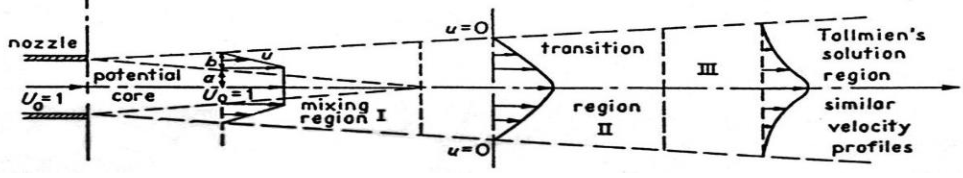
\includegraphics[width=0.95\linewidth]{images/3/getto.png}
    \caption{Rappresentazione dei campi caratteristici di un getto}
\end{figure}

\noindent A partire dalla sezione di uscita vengono a generarsi ed a svilupparsi diverse regioni caratteristiche all'interno di un getto turbolento. In prossimità dell'orifizio si genera una zona conica a velocità costante detta cuore potenziale. Questa zona è delimitata da una mixing region, dove il flusso potenziale si miscela con il flusso circostante. Tale zona è seguita da una zona di transizione ed infine da una zona autosimilare.\\\\
Nella regione autisimilare (o self-similar) il getto evolve rallentando e allargandosi. La peculiarità di questa regione è che i profili di velocità, pur variando in termini assoluti, sono costanti in termini adimensionali purché la normalizzazione venga eseguita in termini di velocità massima e dimensione trasversale del getto locali.

\subsection{Descrizione dell'esperimento}
La presente esercitazione si pone come obiettivo la caratterizzazione della struttura di un getto assialsimmetrico turbolento. Si vuole quindi misurare la velocità media e le fluttuazioni di velocità all'interno del getto, al variare della posizione assiale $x$, della posizione trasversale $r$ e del numero di Reynolds.

\subsection{Catena di misura}
Per misurare la velocità si utilizza un tubo di Pitot, le cui uscite sono collegate al trasduttore di pressione differenziale precedentemente tarato.\\\\
Al fine di misurare la velocità in più punti nello spazio è necessario dotare la catena di misura di alcuni posizionatori. In particolare, il tubo di Pitot è montato su due diverse slitte ortogonali, una che permette il movimento nella direzione assiale e l'altra che permette il movimento nella direzione trasversale.\\\\
La catena di misura è dunque costituita da:
\begin{itemize}
    \item Getto;
    \item Tubo di Pitot;
    \item Posizionatori della sonda di Pitot;
    \item Trasduttore di pressione;
    \item Sistema di acquisizione dati (SAD) e PC con LabView.
\end{itemize}
\begin{figure}[H]
    \centering
    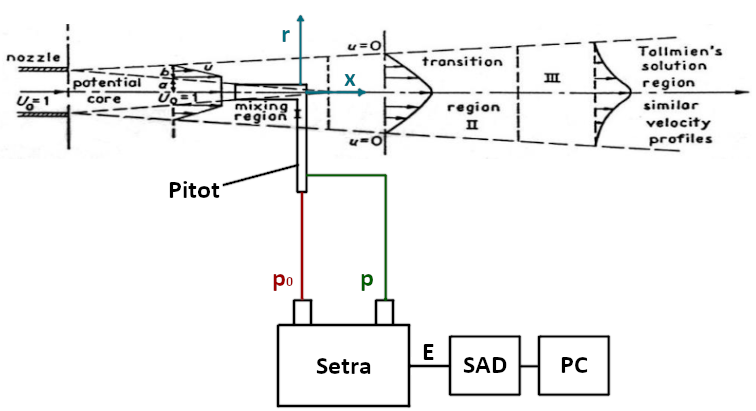
\includegraphics[width=.85\textwidth]{images/3/catena.png}
    \caption{Catena di misura}
\end{figure}
\begin{figure}[H]
    \centering
    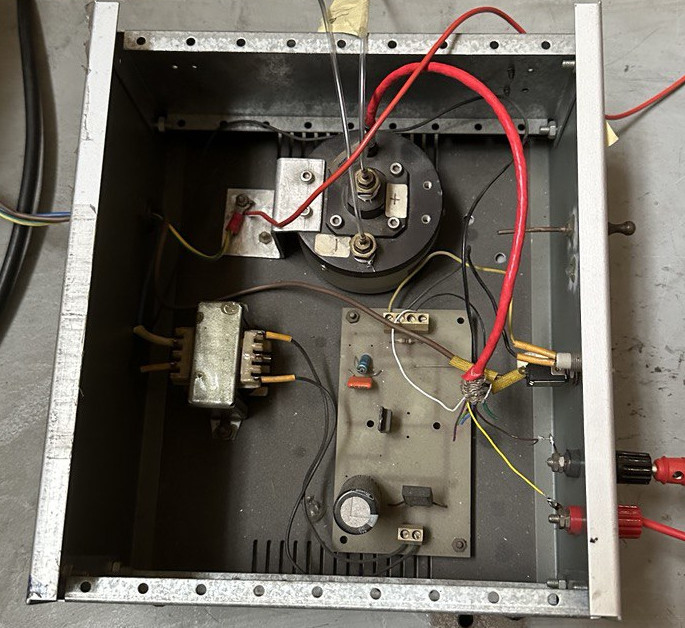
\includegraphics[width=.5\textwidth]{images/3/trasd.jpg}
    \caption{Trasduttore di pressione}
\end{figure}
\begin{figure}[ht]
    \centering
    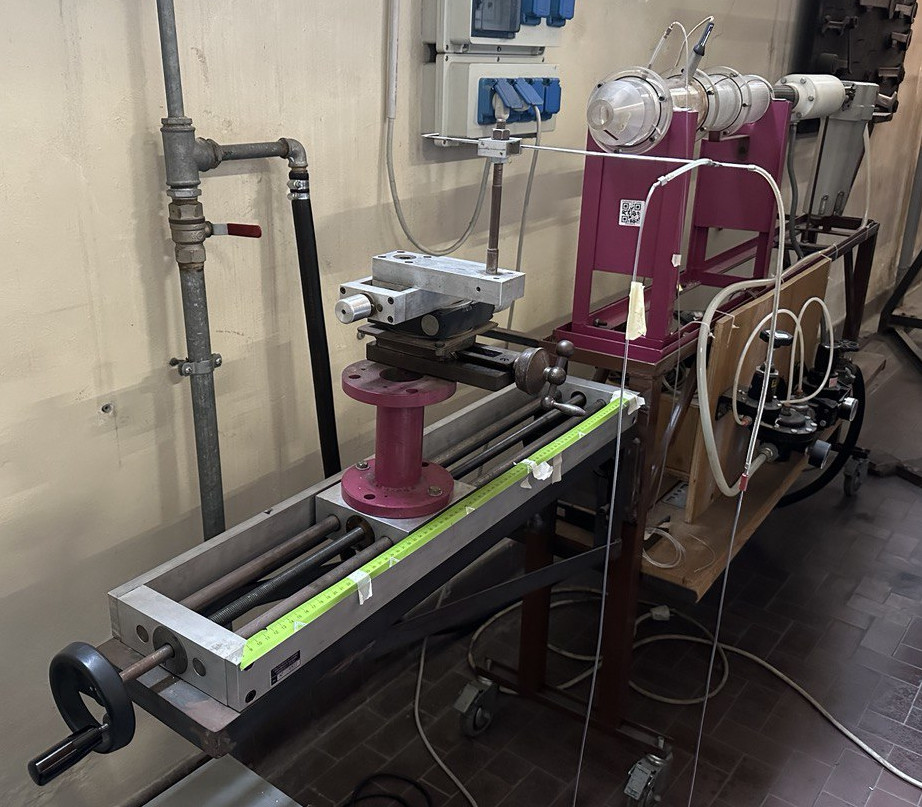
\includegraphics[width=.85\textwidth]{images/3/gettomanopole.jpg}
    \caption{Sistema di posizionamento della sonda di Pitot}
\end{figure}

\subsection{Procedimento operativo}
Ogni squadra effettua misure per una portata costante. Pertanto si ricavano dati per quattro diversi valori di portata, quindi quattro diversi numeri di Reynolds.\\\\
Le misure sono effettuate al variare della distanza trasversale del getto $r$ e per diversi valori di distanza assiale $x$.\\\\
Per regolare la distanza trasversale e la distanza assiale, sono presenti due diverse manopole. Il primo passo consiste nel misurare l'attuale distanza assiale con l'utilizzo di un metro. Una volta definita la distanza assiale, si procede a far variare la distanza trasversale in entrambi i versi rispetto all'asse del getto e si acquisiscono i dati in uscita dal trasduttore di pressione. Una volta acquisiti sufficienti misurazioni si passa ad una diversa distanza assiale $x$ e si ripete la procedura di acquisizione dati.\\\\
I dati grezzi acquisiti mediante questa procedura sono riportati in appendice \ref{a3}.

\subsection{Analisi dati}
L'analisi dati è condotta con l'ausilio di un codice Python, riportato in appendice \ref{b3}.\\\\
Come prima cosa si utilizzano i valori di pressione e temperatura ambiente per determinare la densità e la viscosità dinamica dell'aria:
\begin{equation*}
    \rho = \frac{p_{amb}}{R T_{amb}} \qquad \mu = 1.46\cdot10^{-6} \frac{T_{amb}^{3/2}}{T_{amb}+110}
\end{equation*}
Successivamente si misura la tensione di offset del trasduttore $E_0$, così da poter scomporre il segnale di tensione in uscita come segue:
\begin{equation*}
    E = E_0 + \Delta E
\end{equation*}
Dalle tensioni in uscita acquisite, si calcola la pressione dinamica e quindi la velocità:
\begin{equation*}
    q = \frac12 \rho U^2 = K_t \Delta E = K_t (E - E_0) \quad \Rightarrow \quad U = \sqrt{\frac{2q}\rho}
\end{equation*}
Si può quindi diagrammare l'andamento della velocità in funzione della posizione trasversale $r$ ed assiale $x$:
\begin{figure}[h]
    \centering
    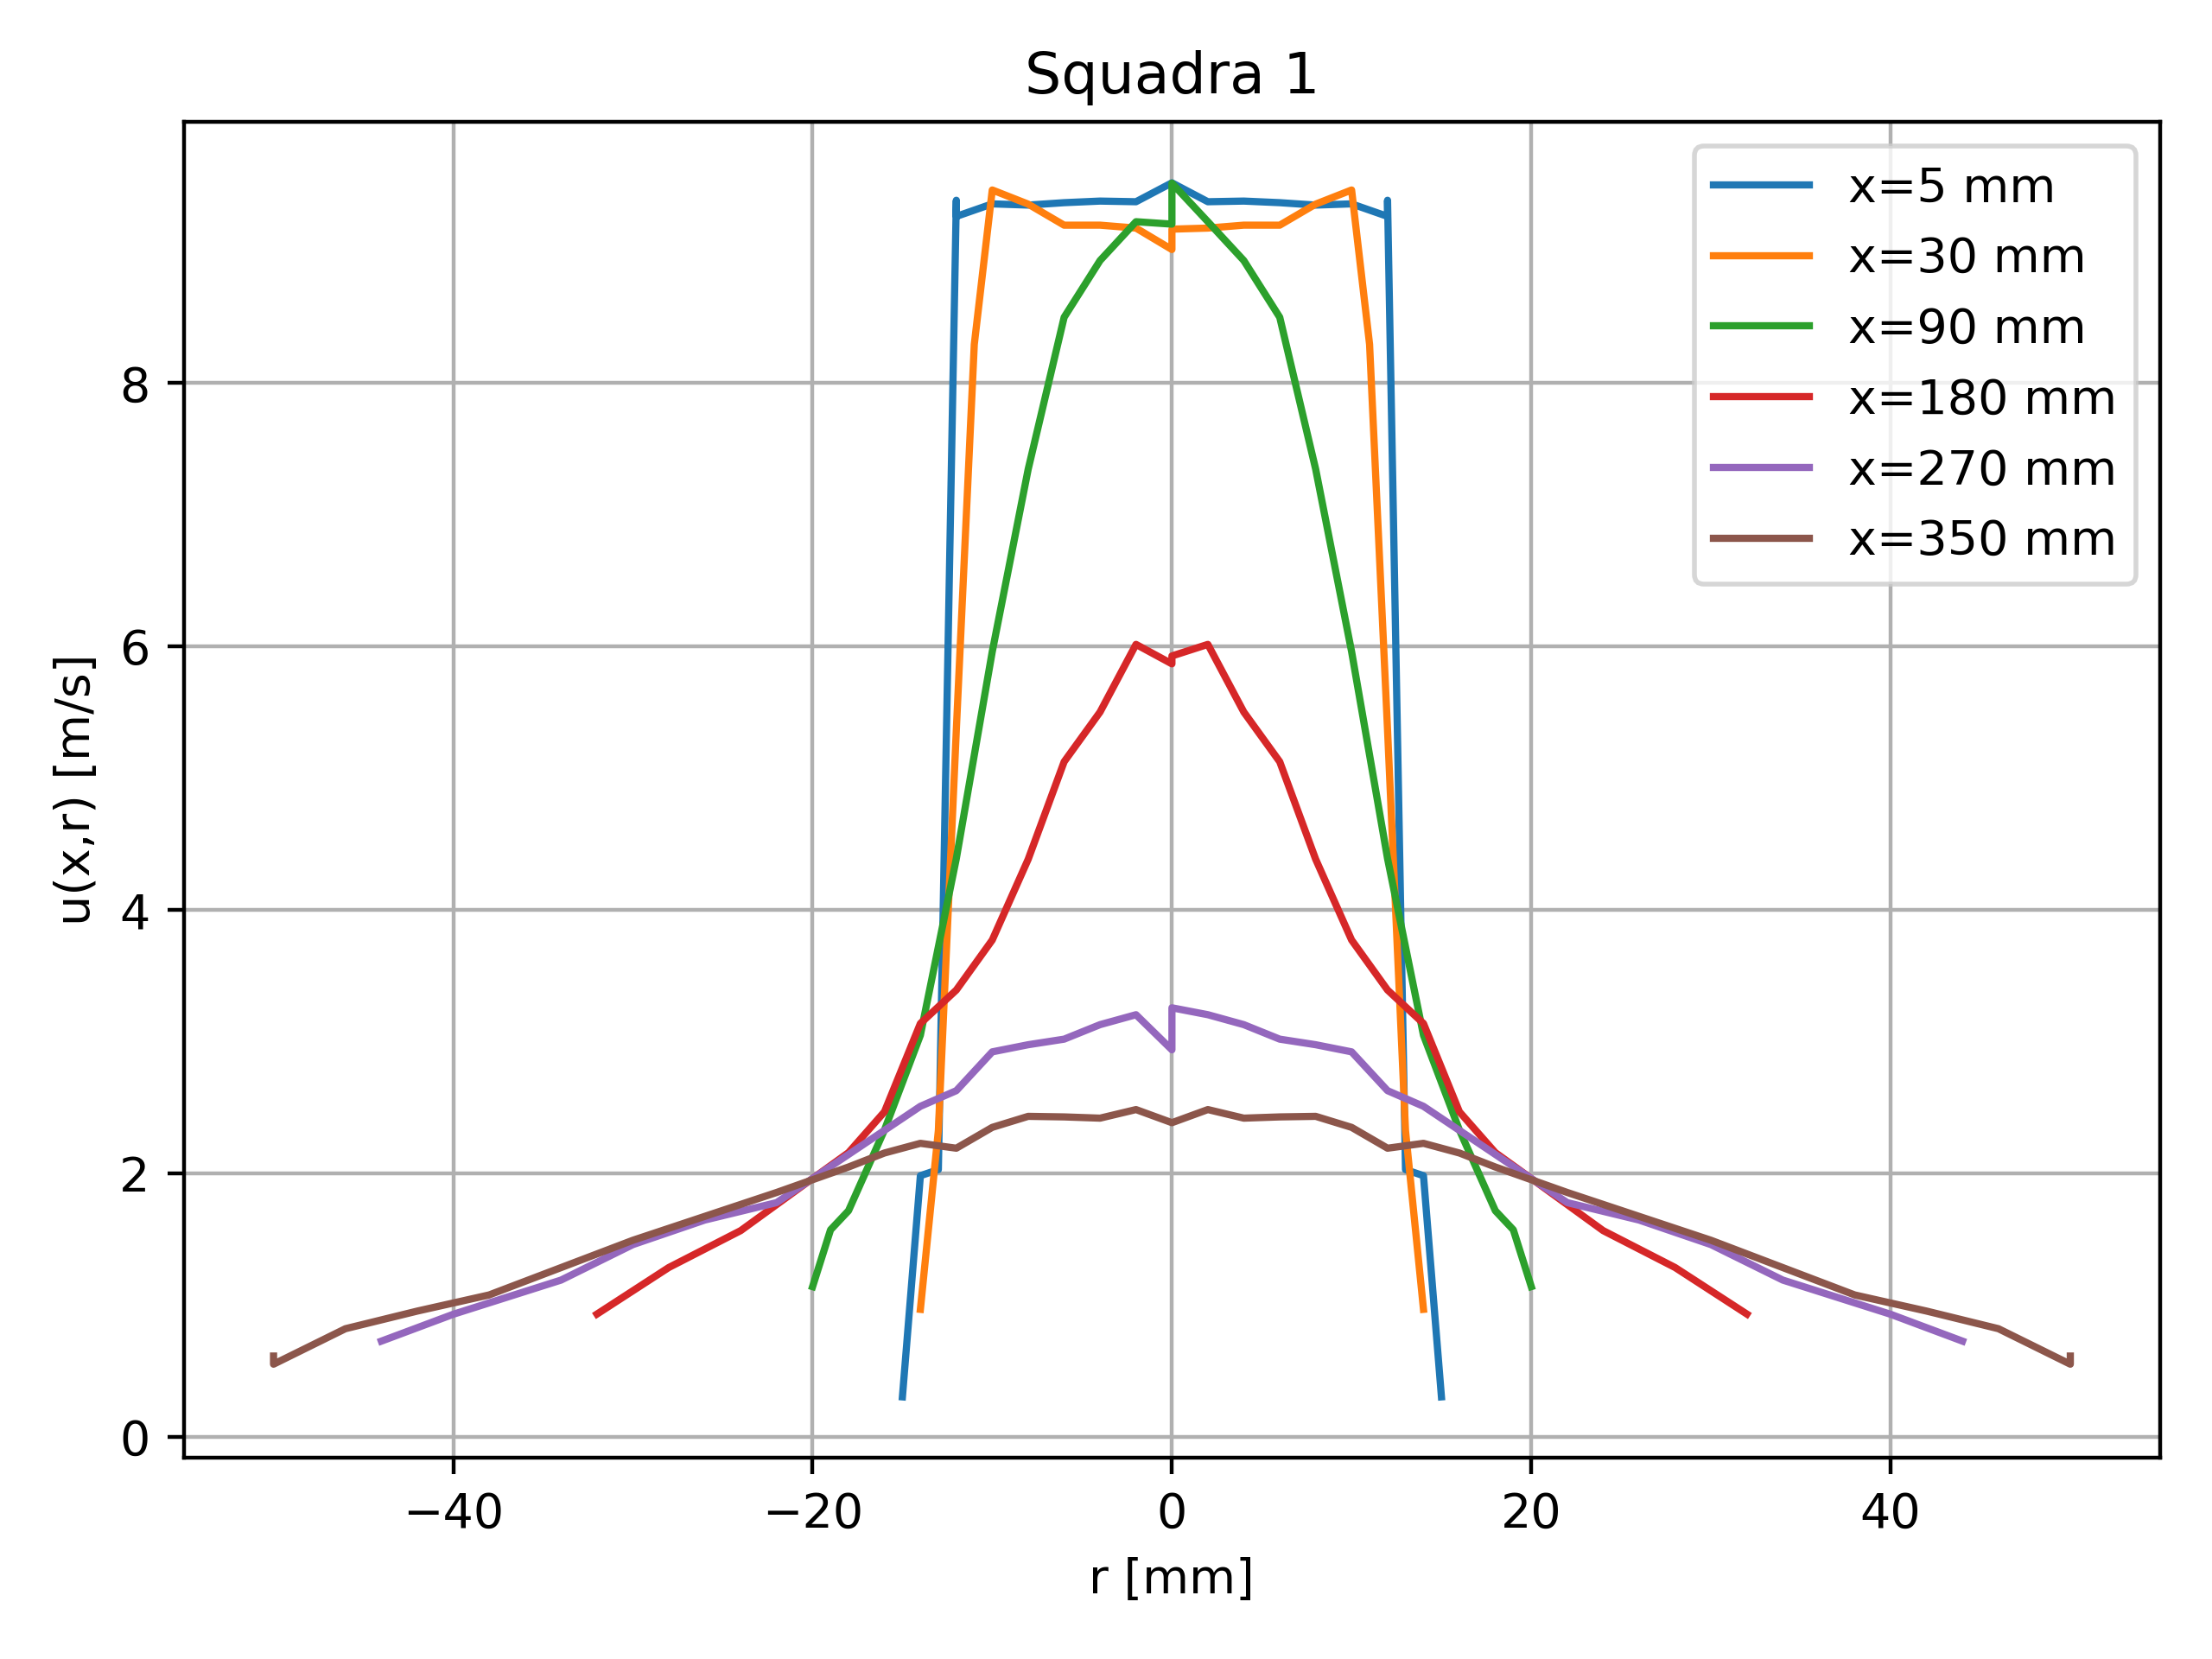
\includegraphics[width=.9\textwidth]{images/3/sq1.png}
    \caption{Profili di velocità per la prima squadra}
\end{figure}
\begin{figure}[ht]
    \centering
    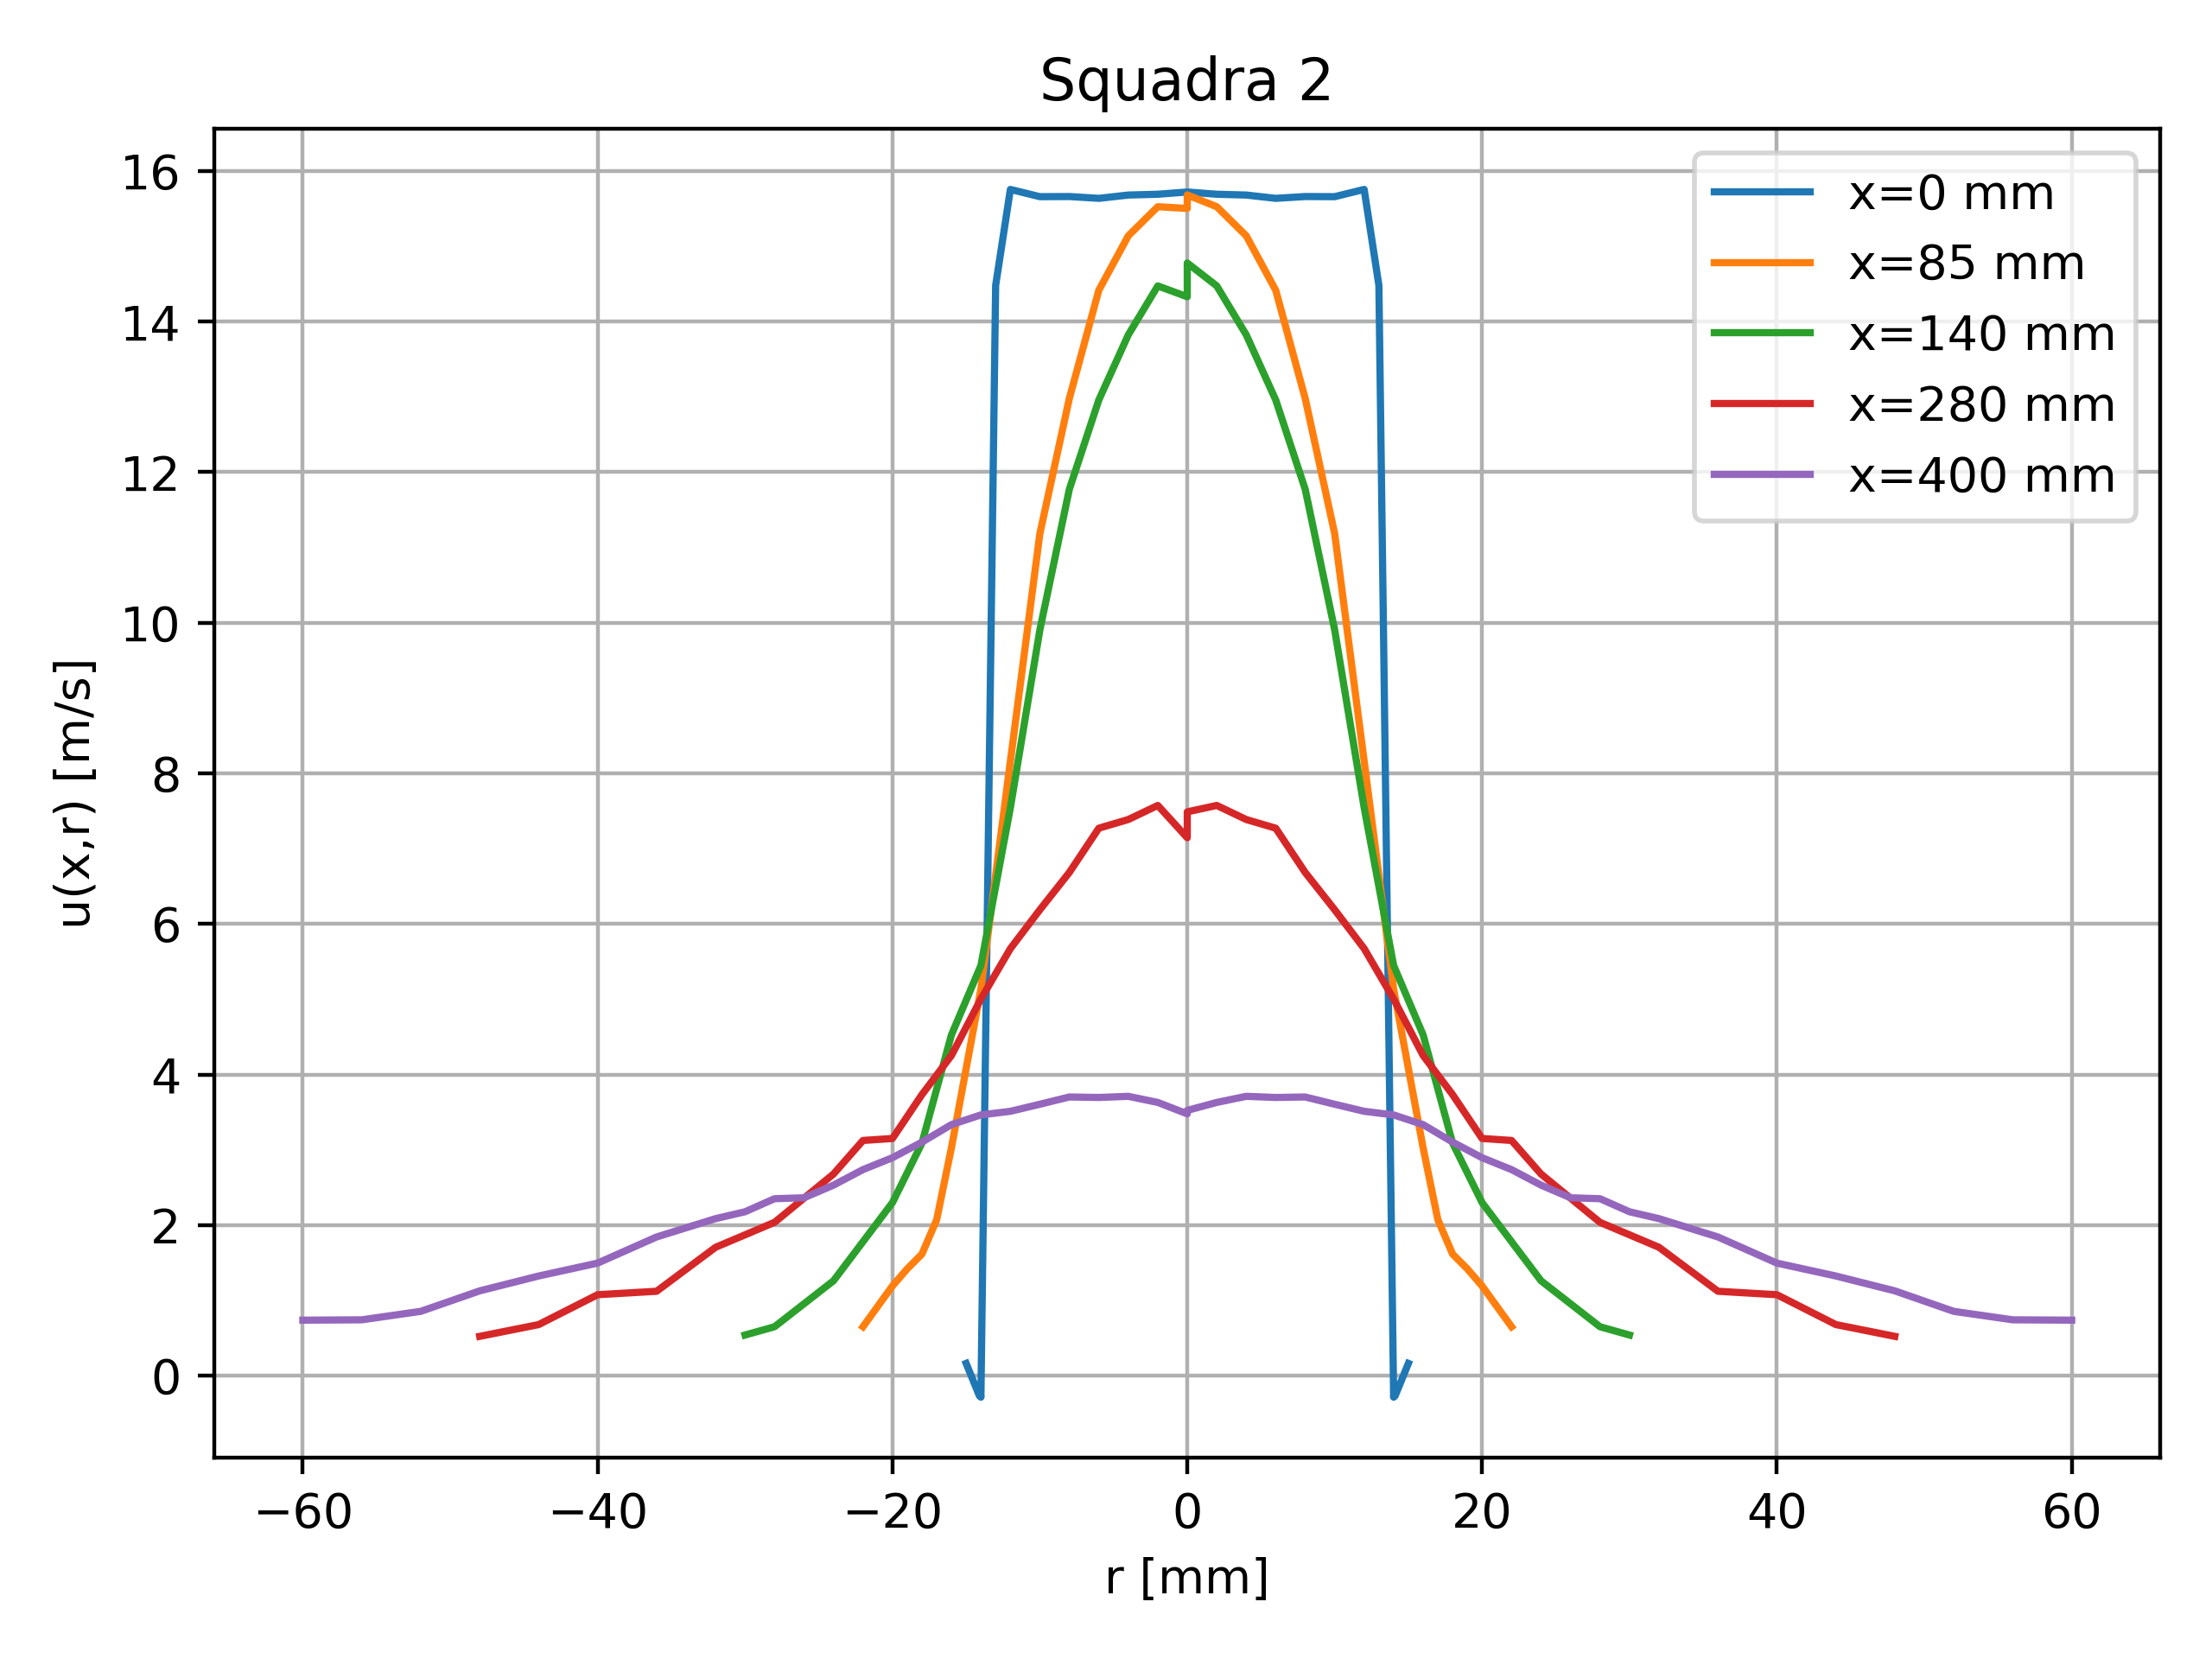
\includegraphics[width=.85\textwidth]{images/3/sq2.png}
    \caption{Profili di velocità per la seconda squadra}
\end{figure}
\begin{figure}[H]
    \centering
    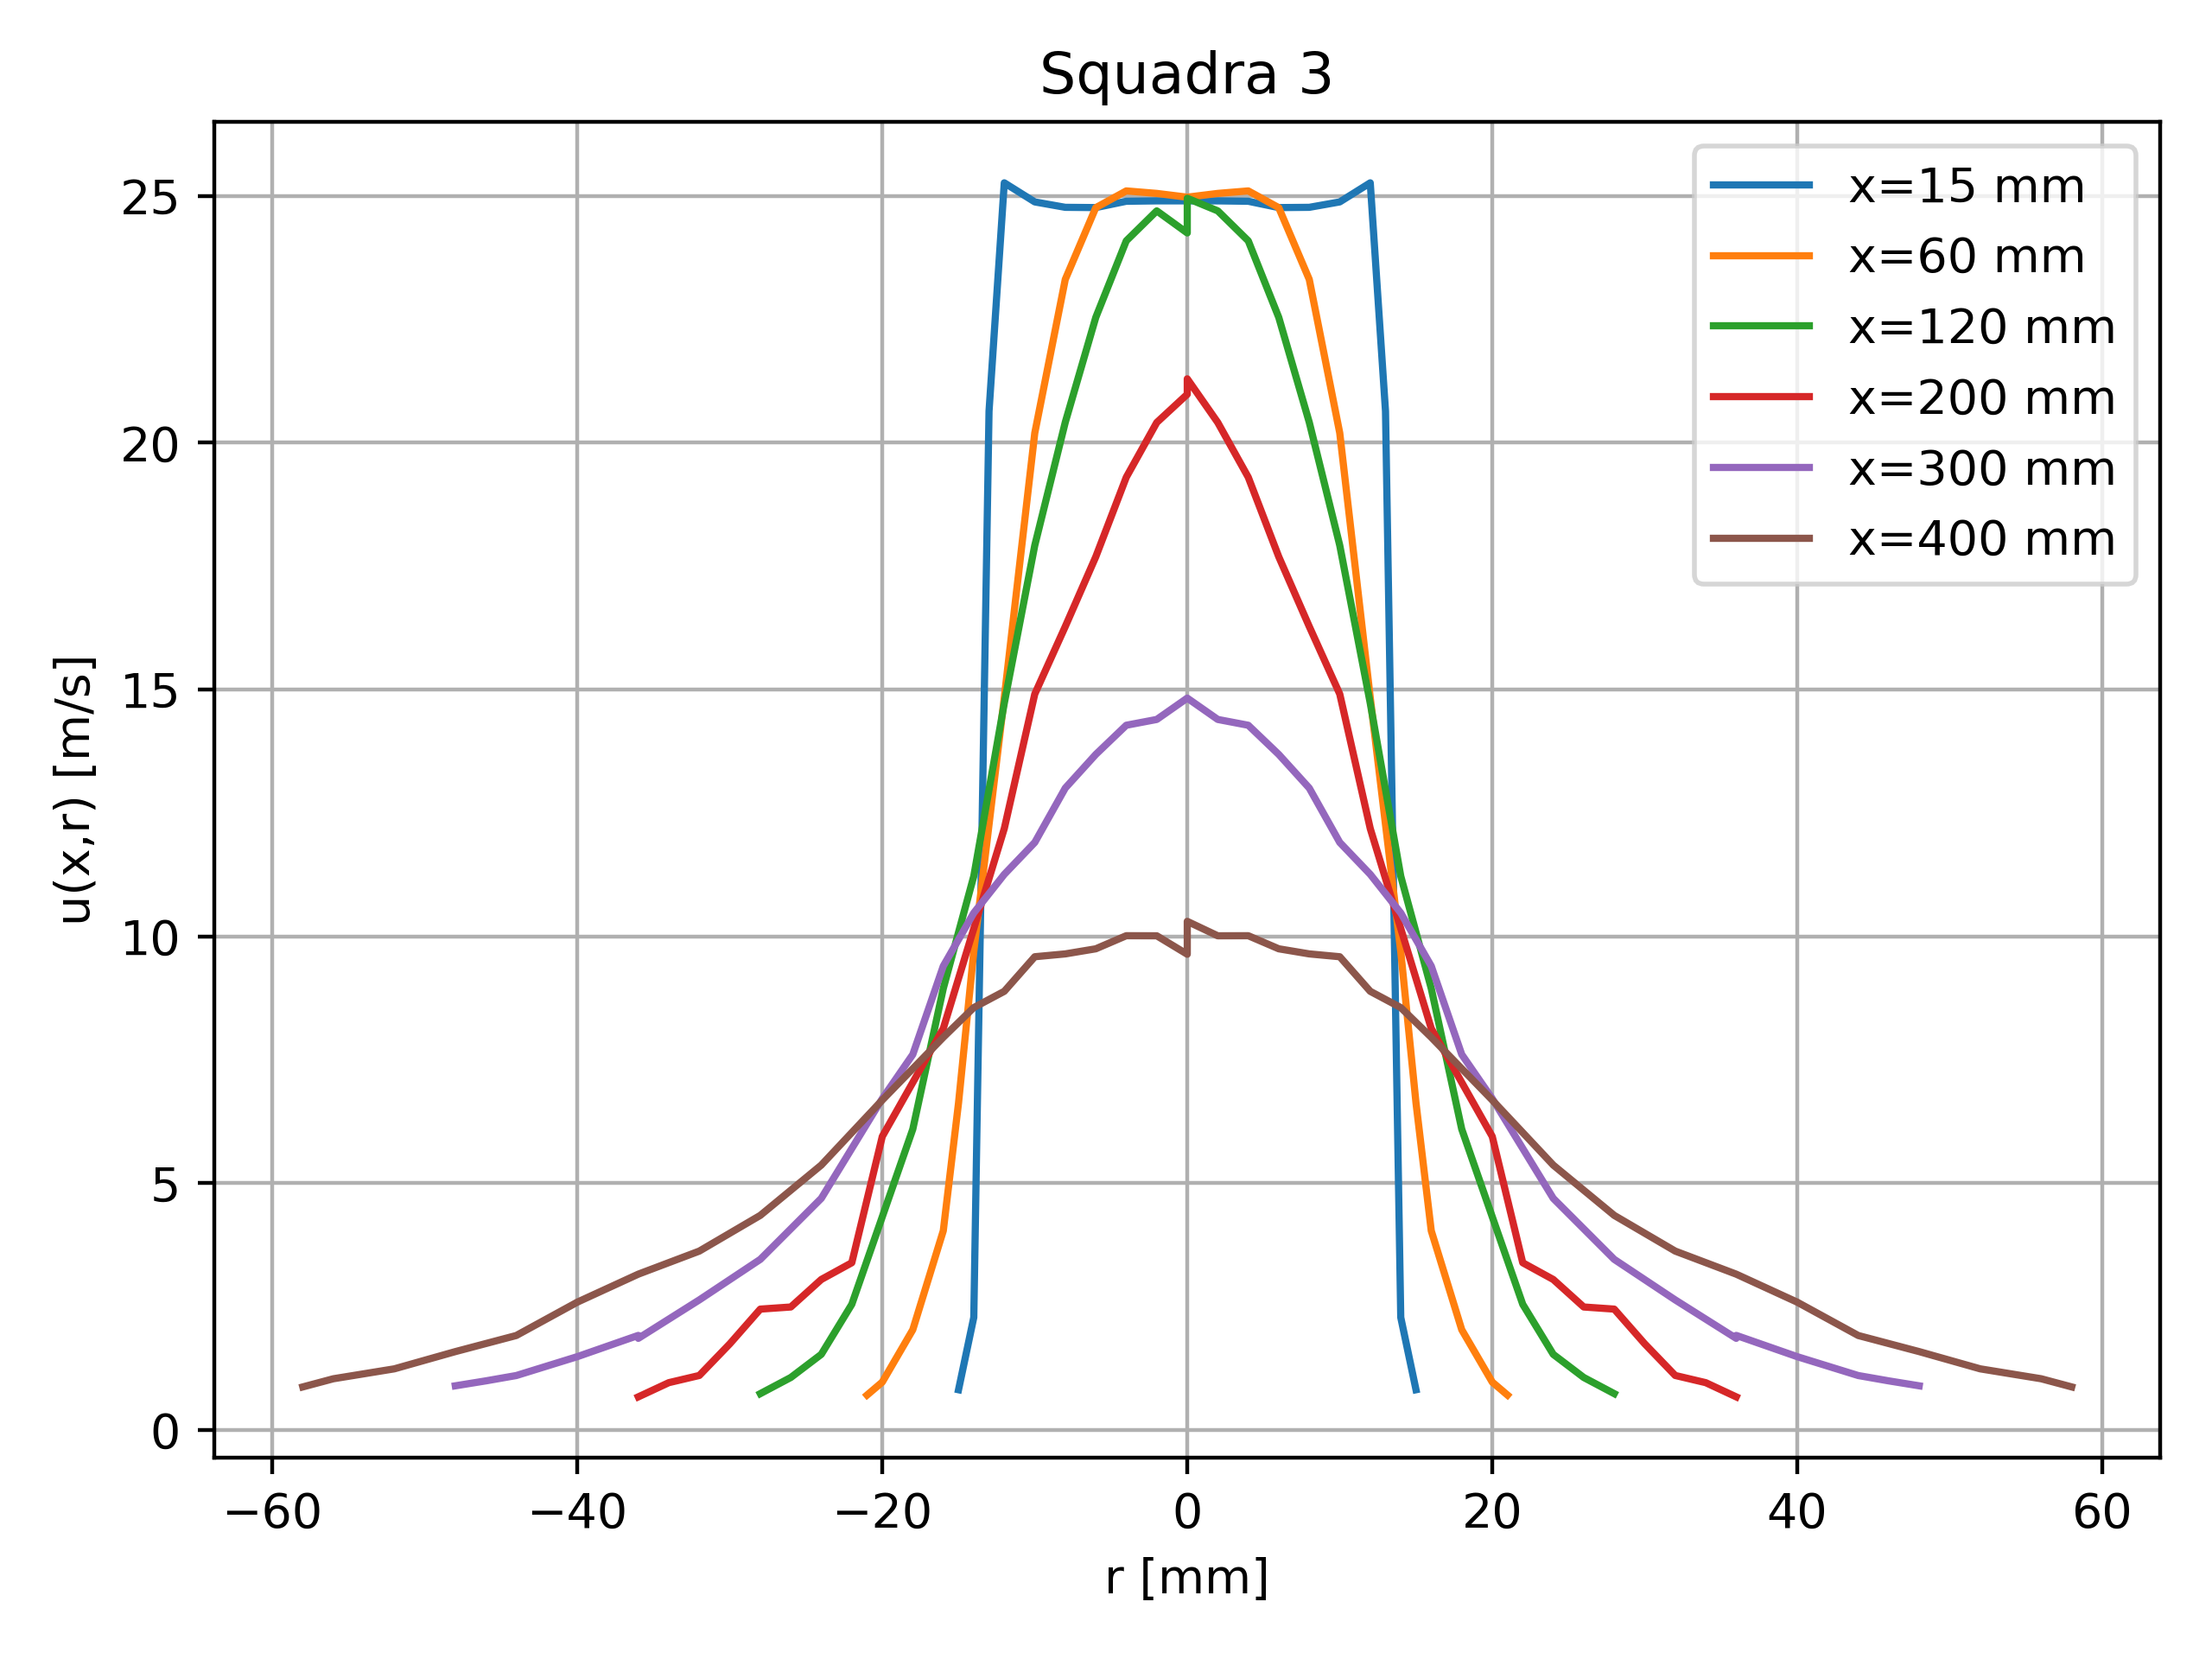
\includegraphics[width=.85\textwidth]{images/3/sq3.png}
    \caption{Profili di velocità per la terza squadra}
\end{figure}
\begin{figure}[ht]
    \centering
    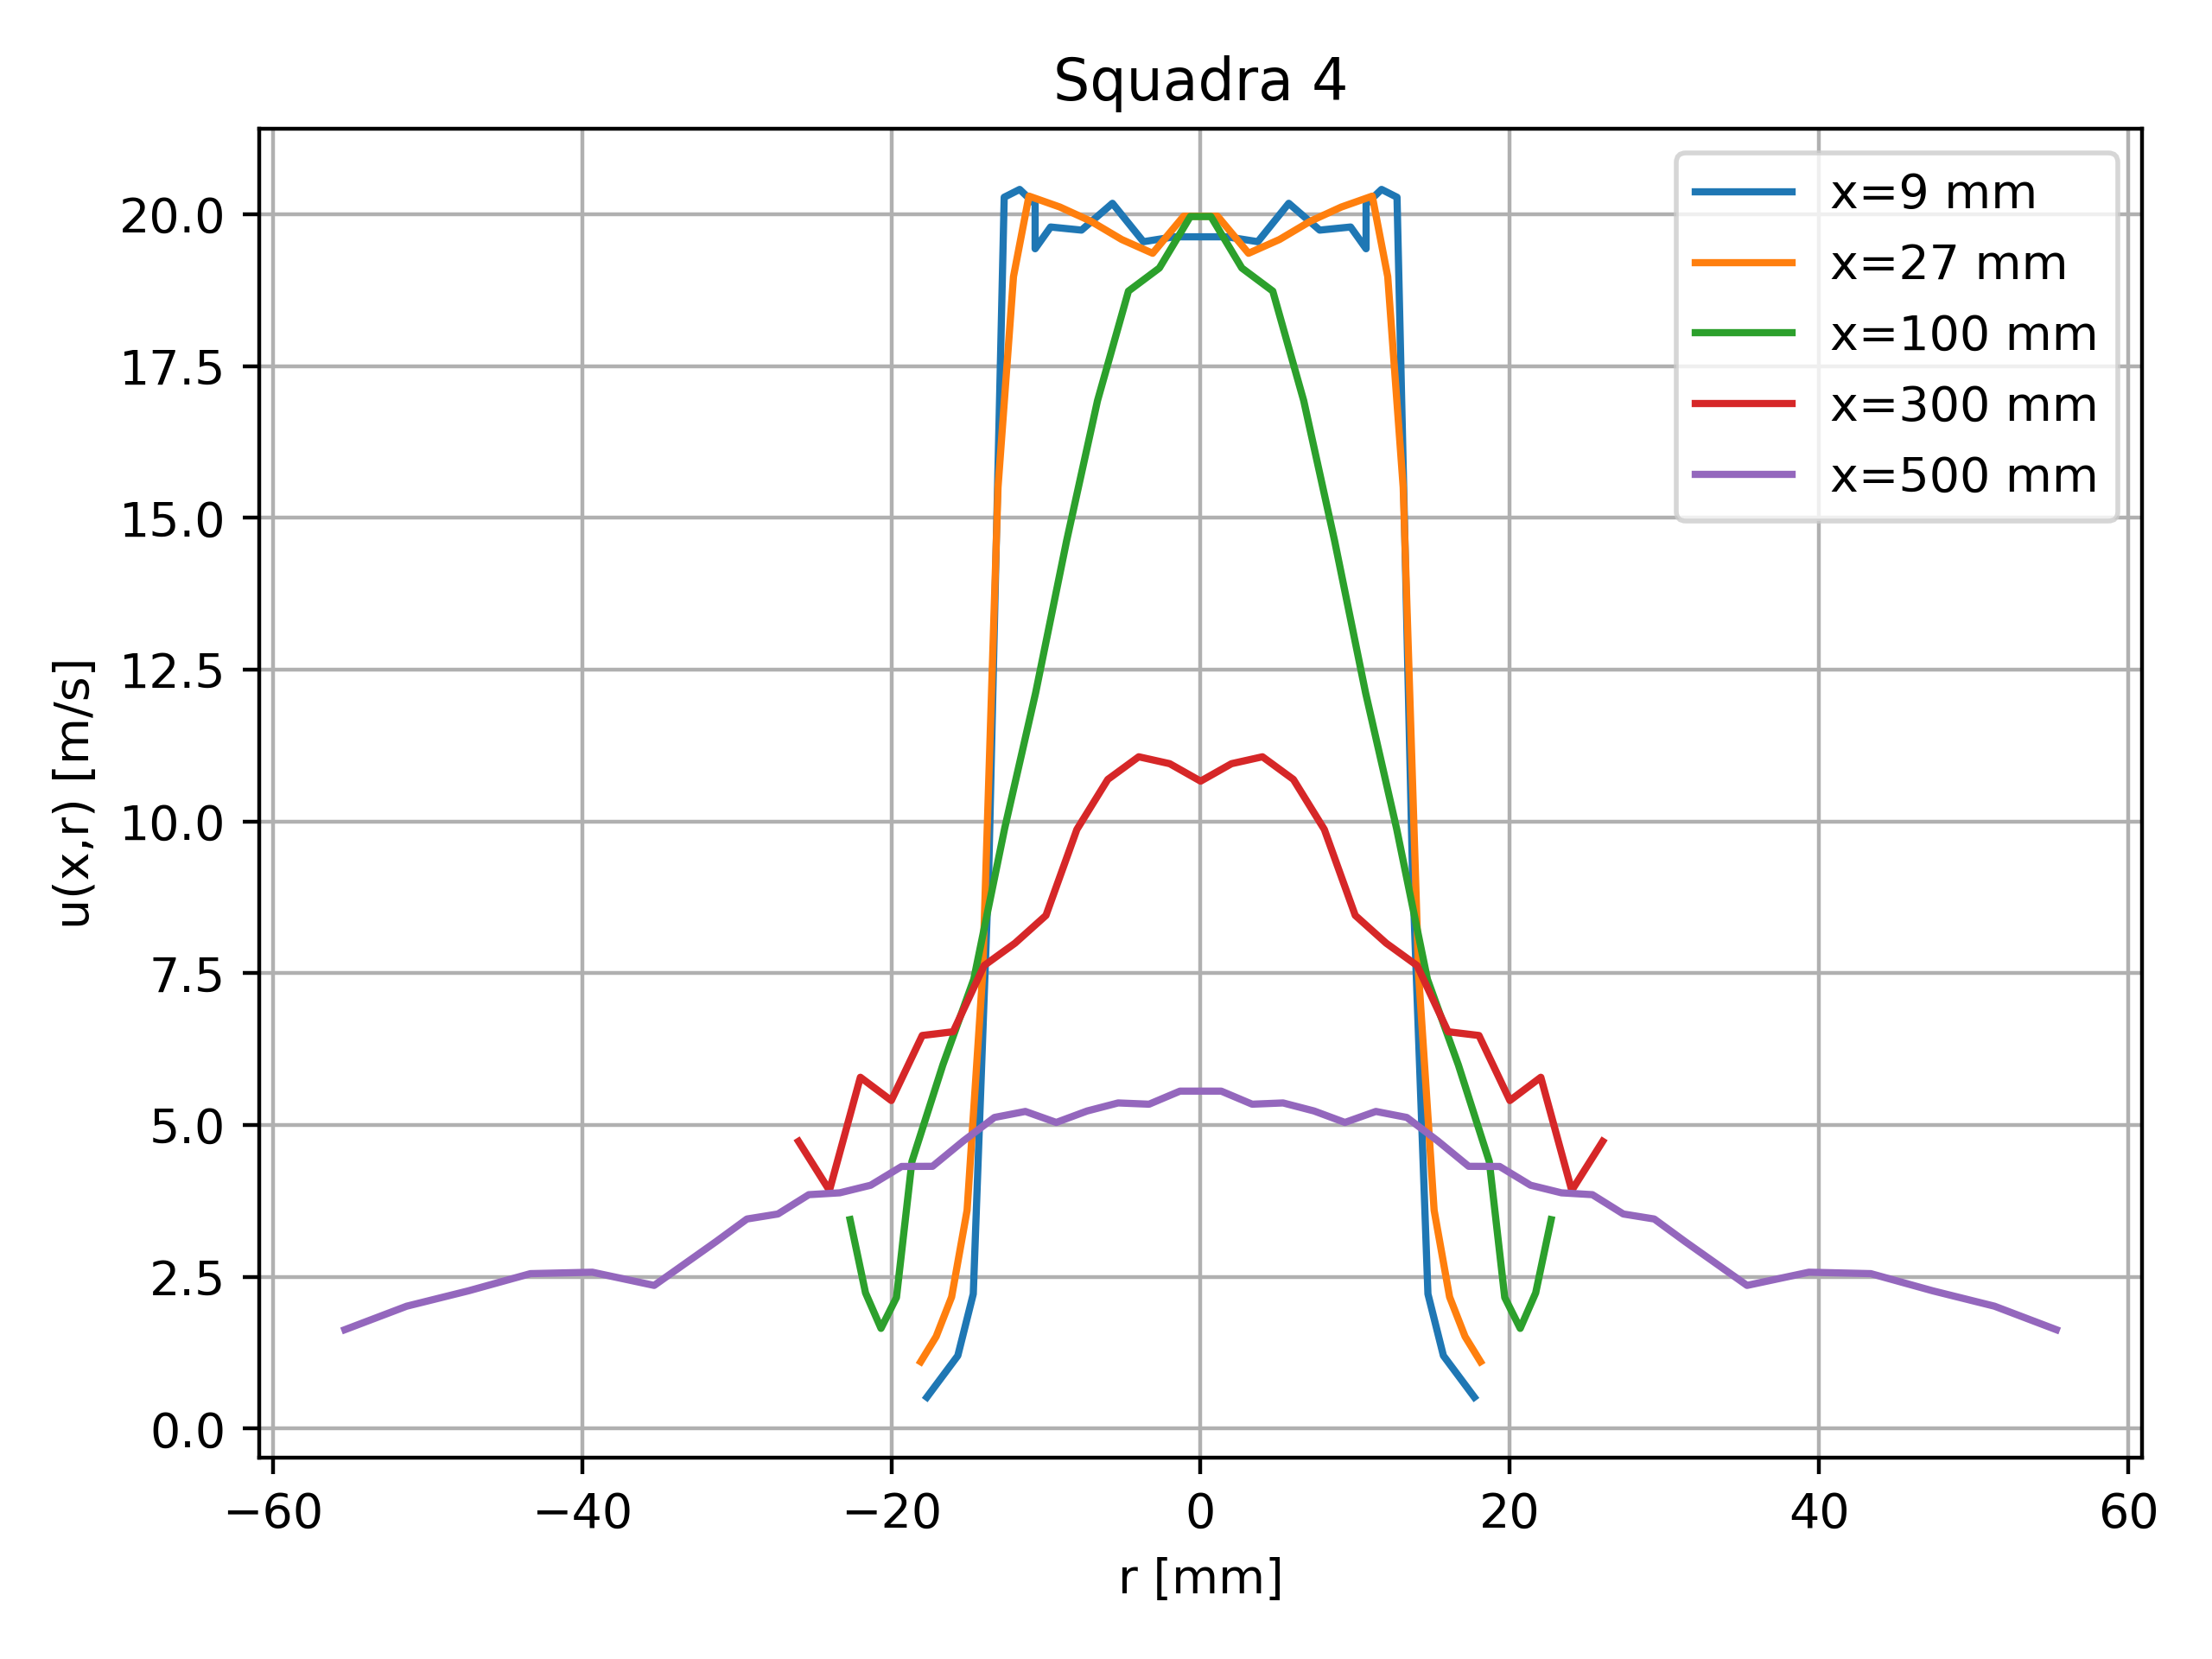
\includegraphics[width=.8\textwidth]{images/3/sq4.png}
    \caption{Profili di velocità per la quarta squadra}
\end{figure}

\noindent Per una migliore interpretazione, tali diagrammi possono essere visualizzati in uno spazio tridimensionale, così da esplicitare la distanza assiale $x$:
\begin{figure}[H]
    \centering
    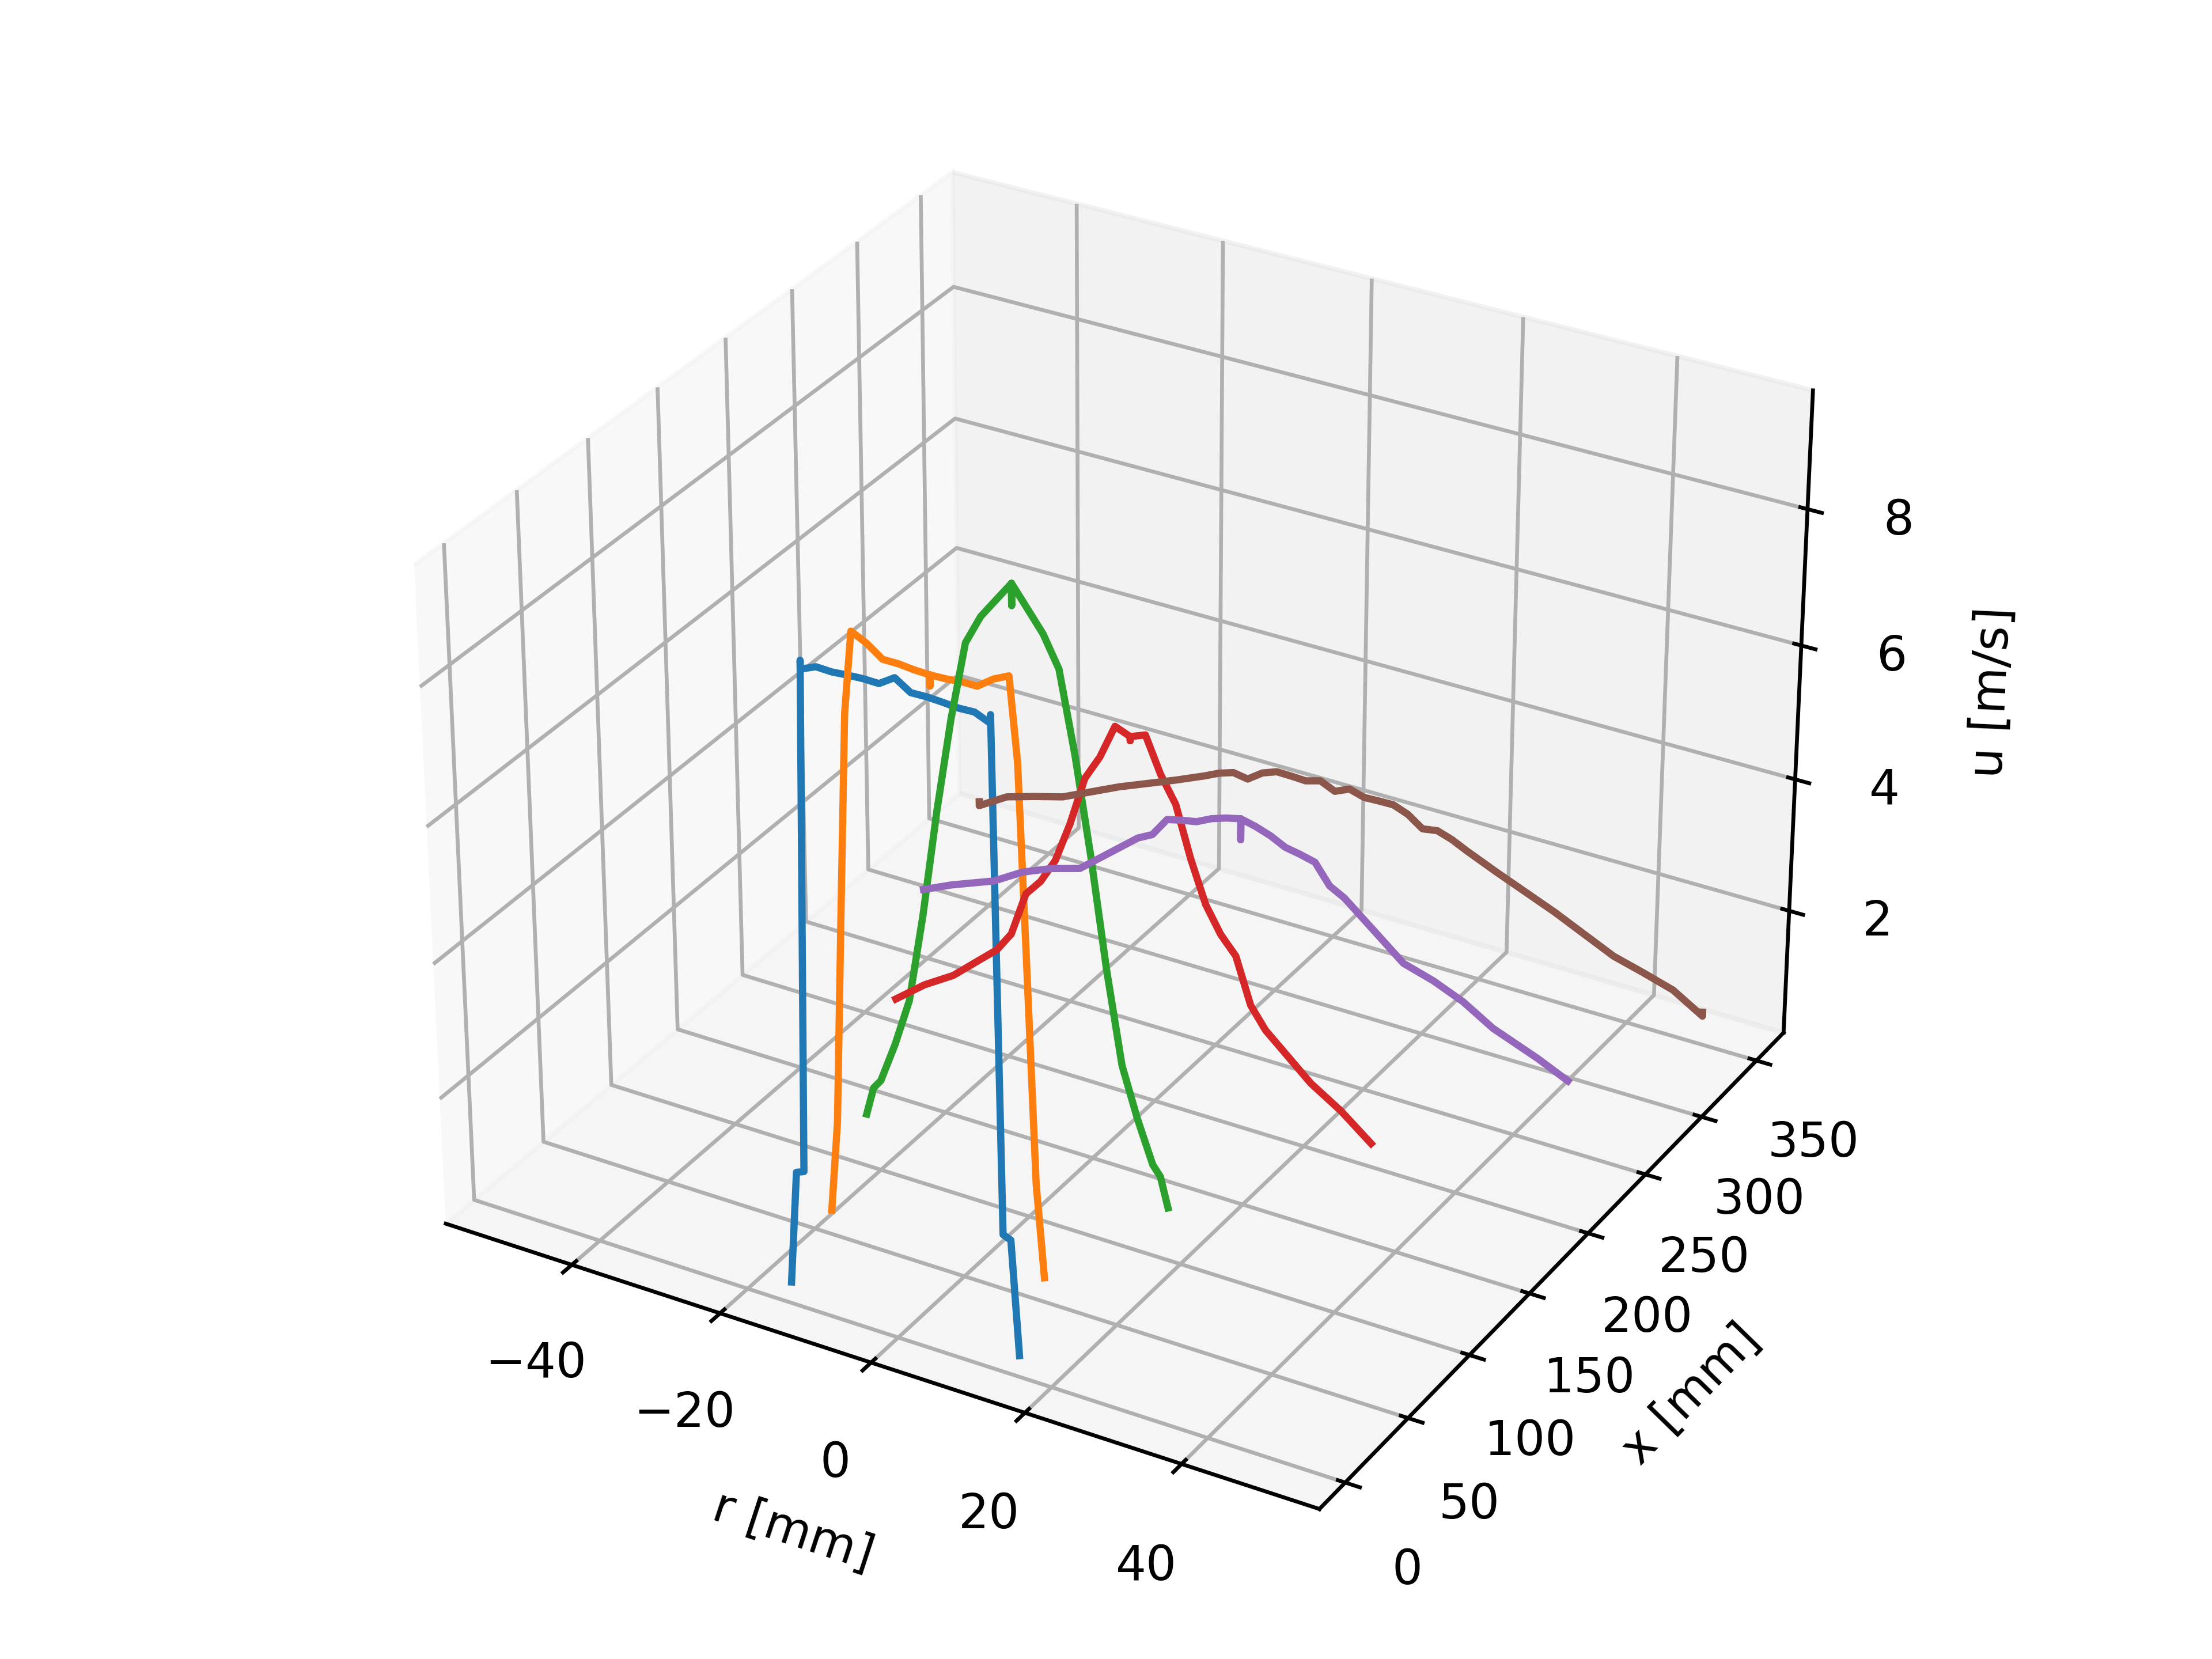
\includegraphics[width=.8\textwidth]{images/3/sq13d.png}
    \caption{Profili di velocità per la prima squadra}
\end{figure}
\begin{figure}[H]
    \centering
    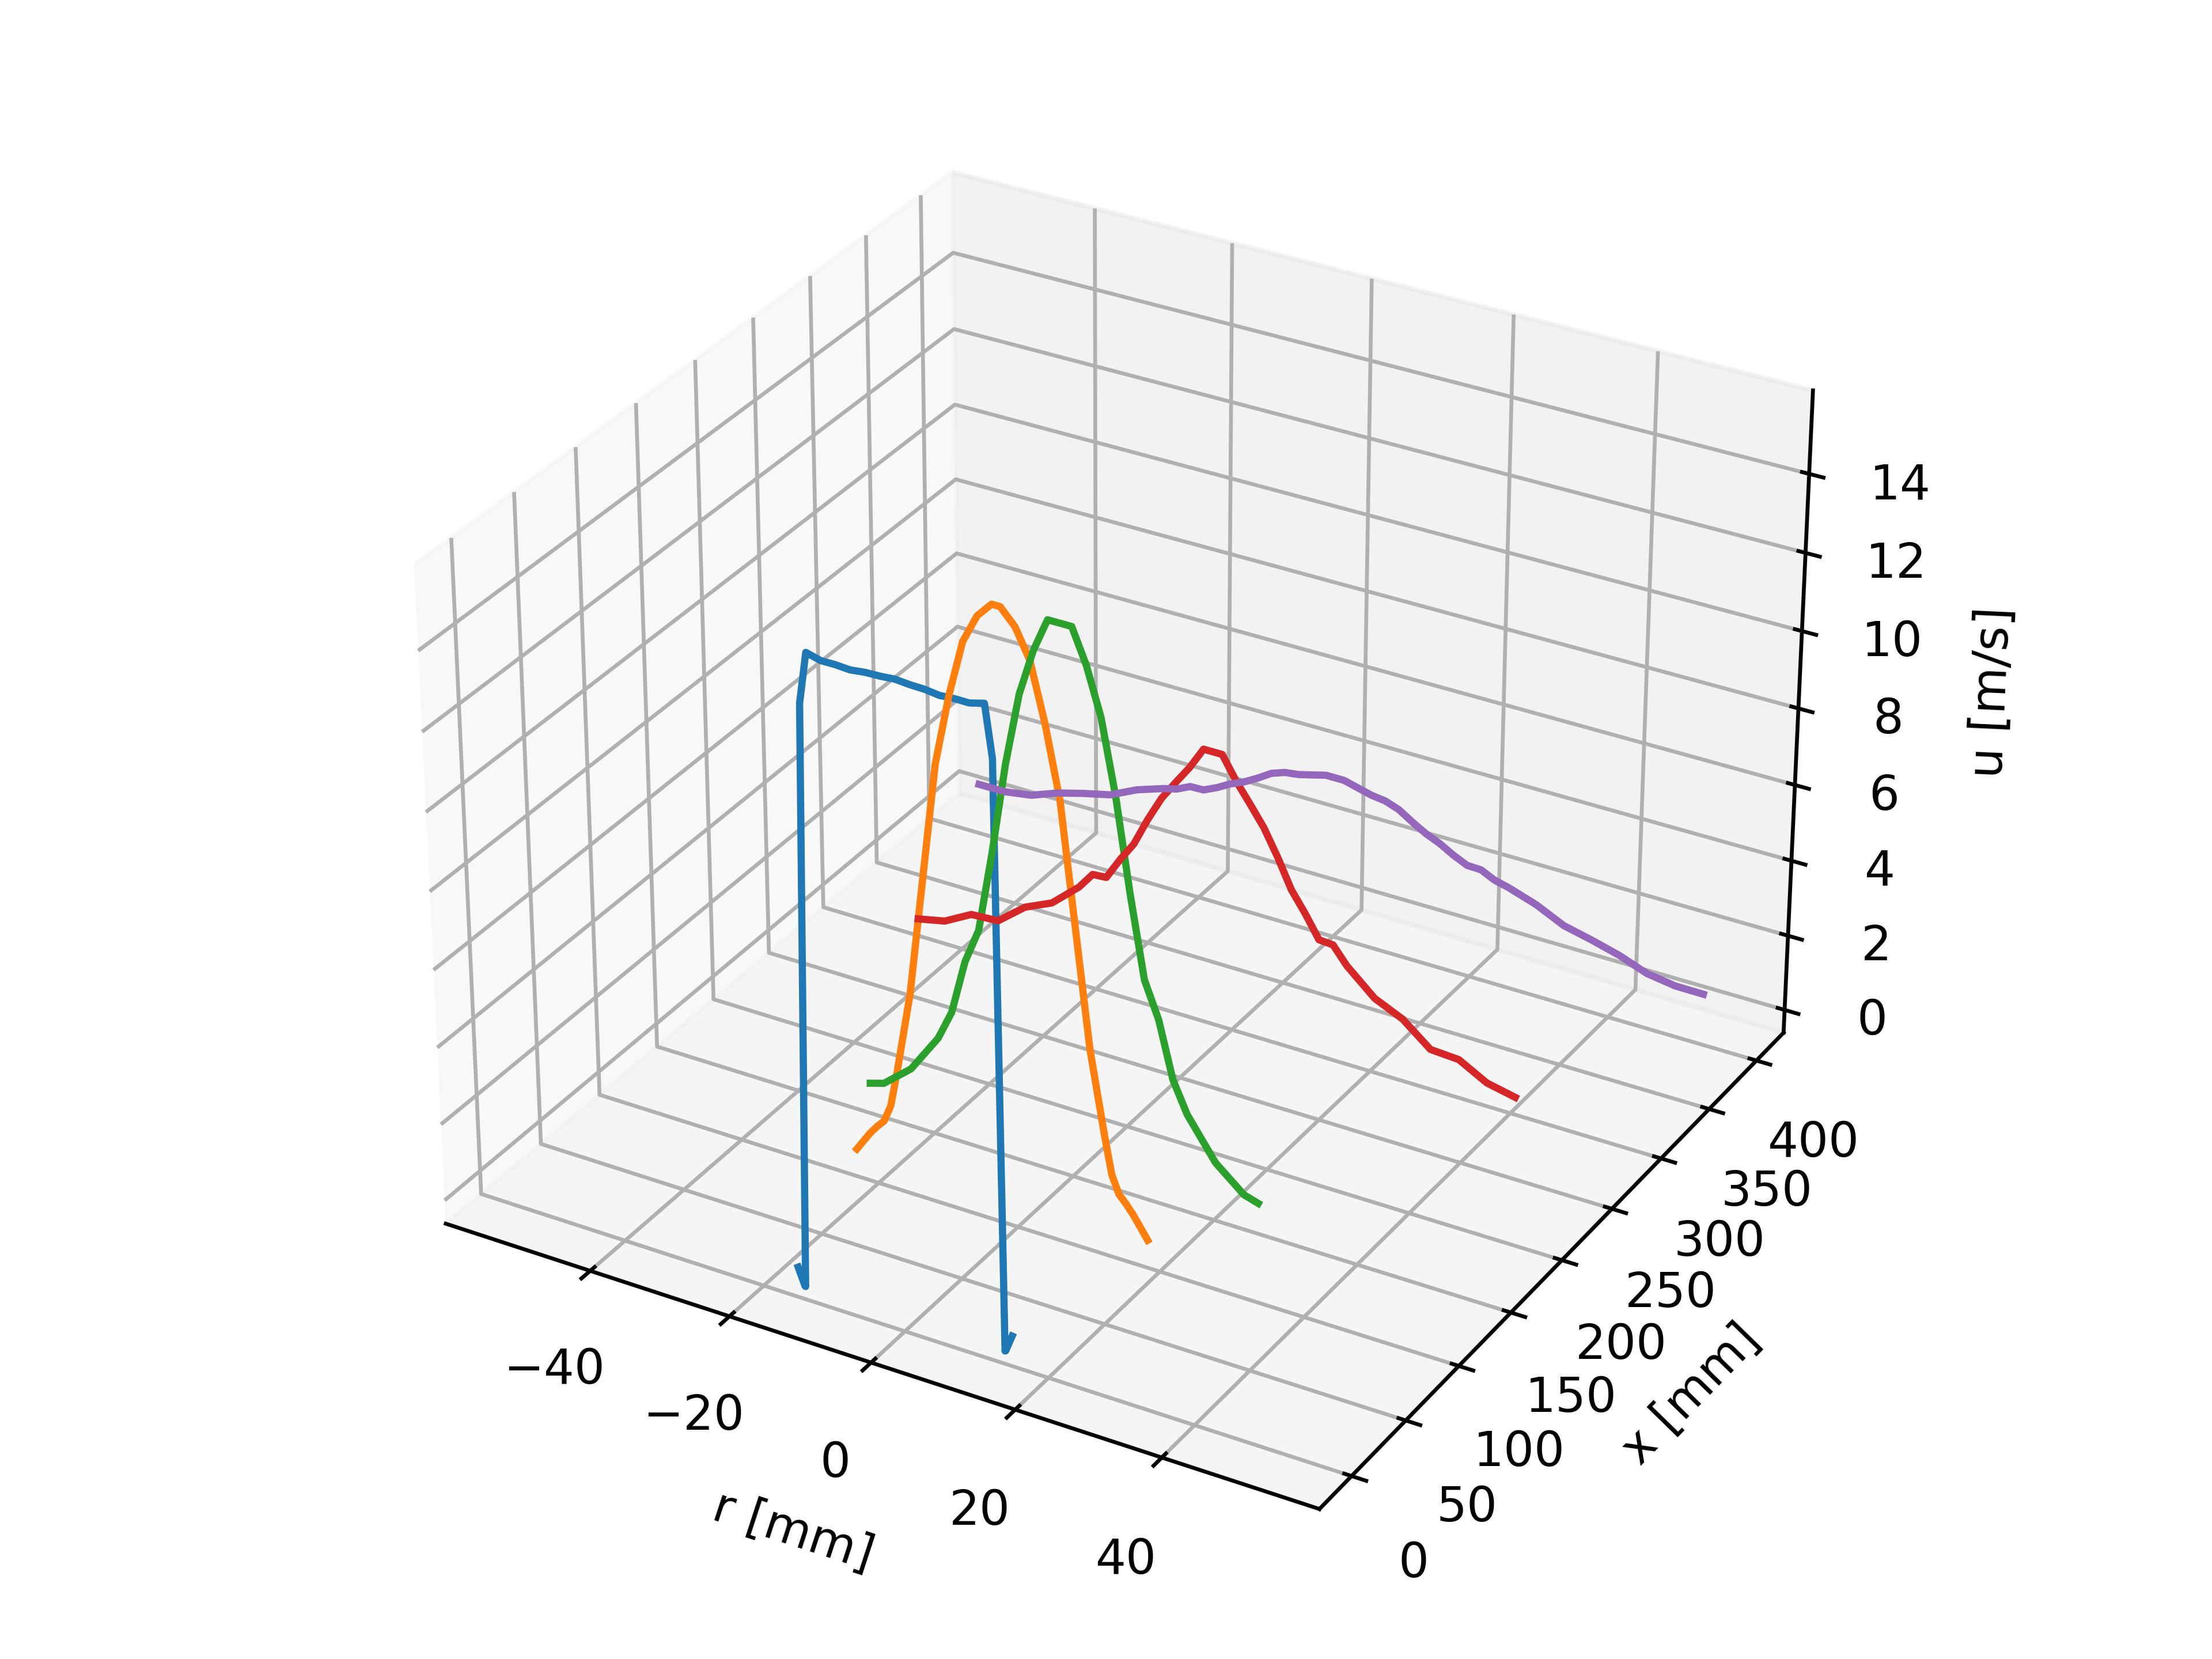
\includegraphics[width=.92\textwidth]{images/3/sq23d.png}
    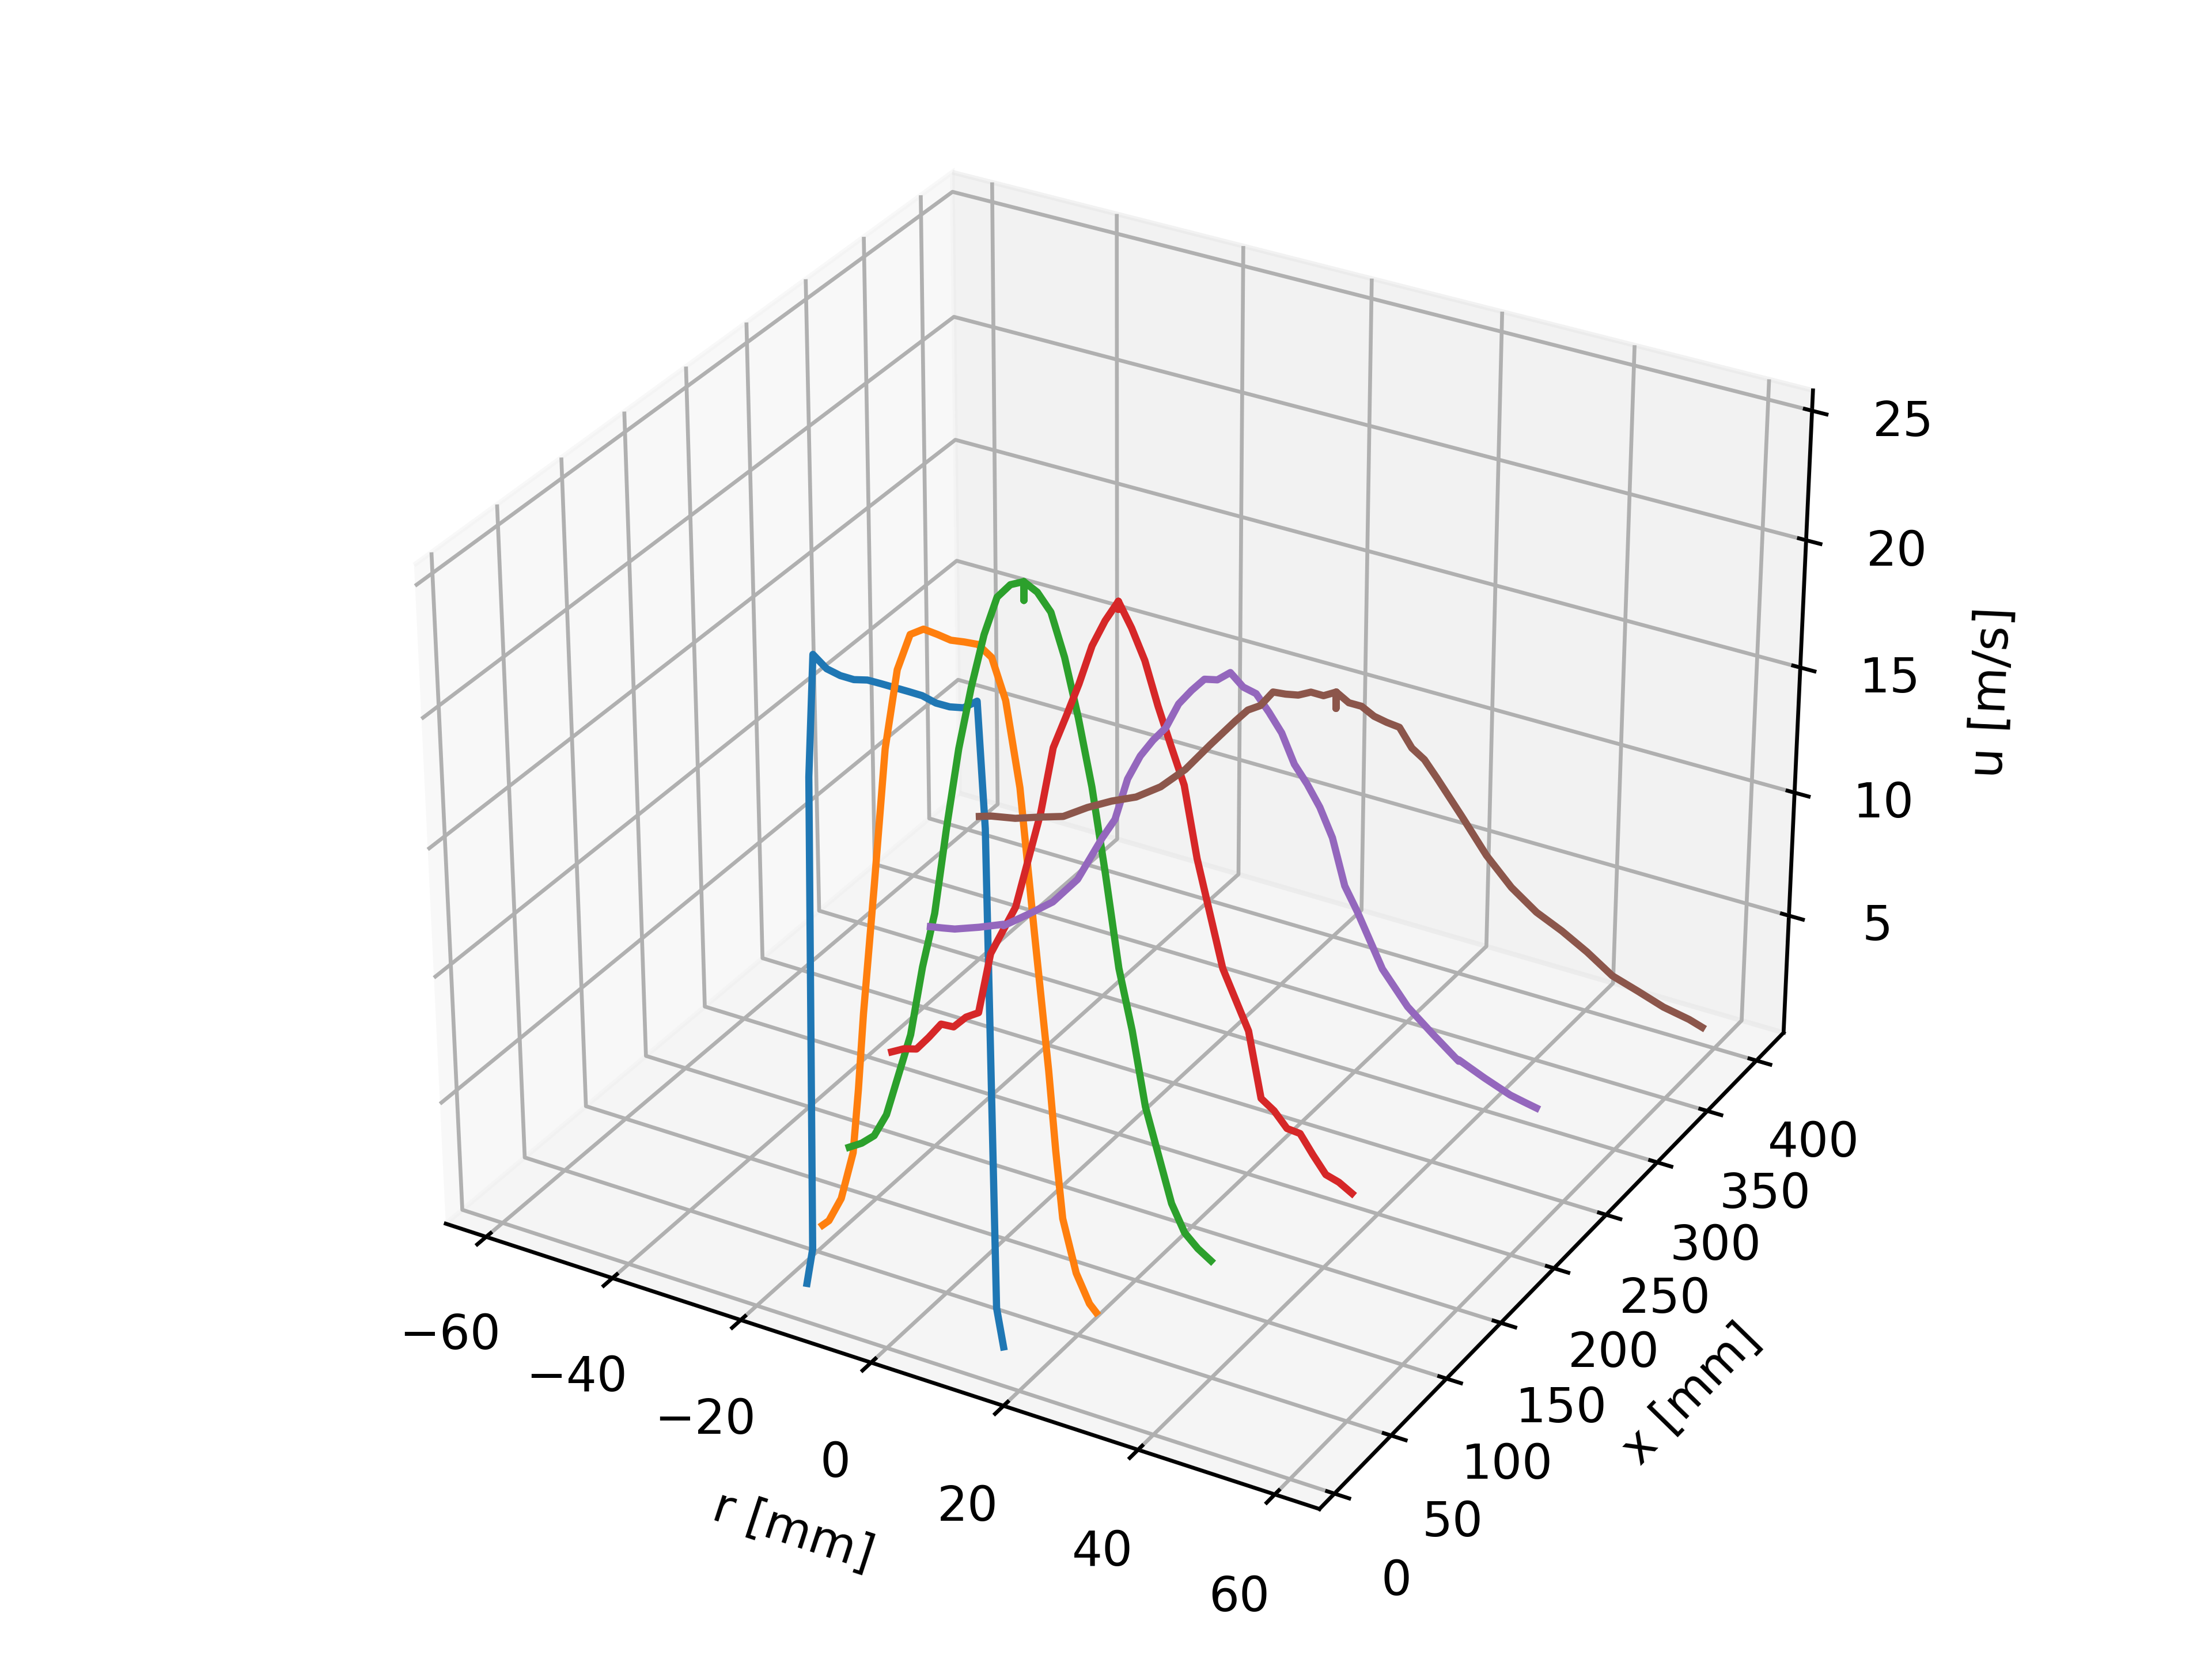
\includegraphics[width=.92\textwidth]{images/3/sq33d.png}
    \caption{Profili di velocità per la seconda e per la terza squadra}
\end{figure}
\begin{figure}[H]
    \centering
    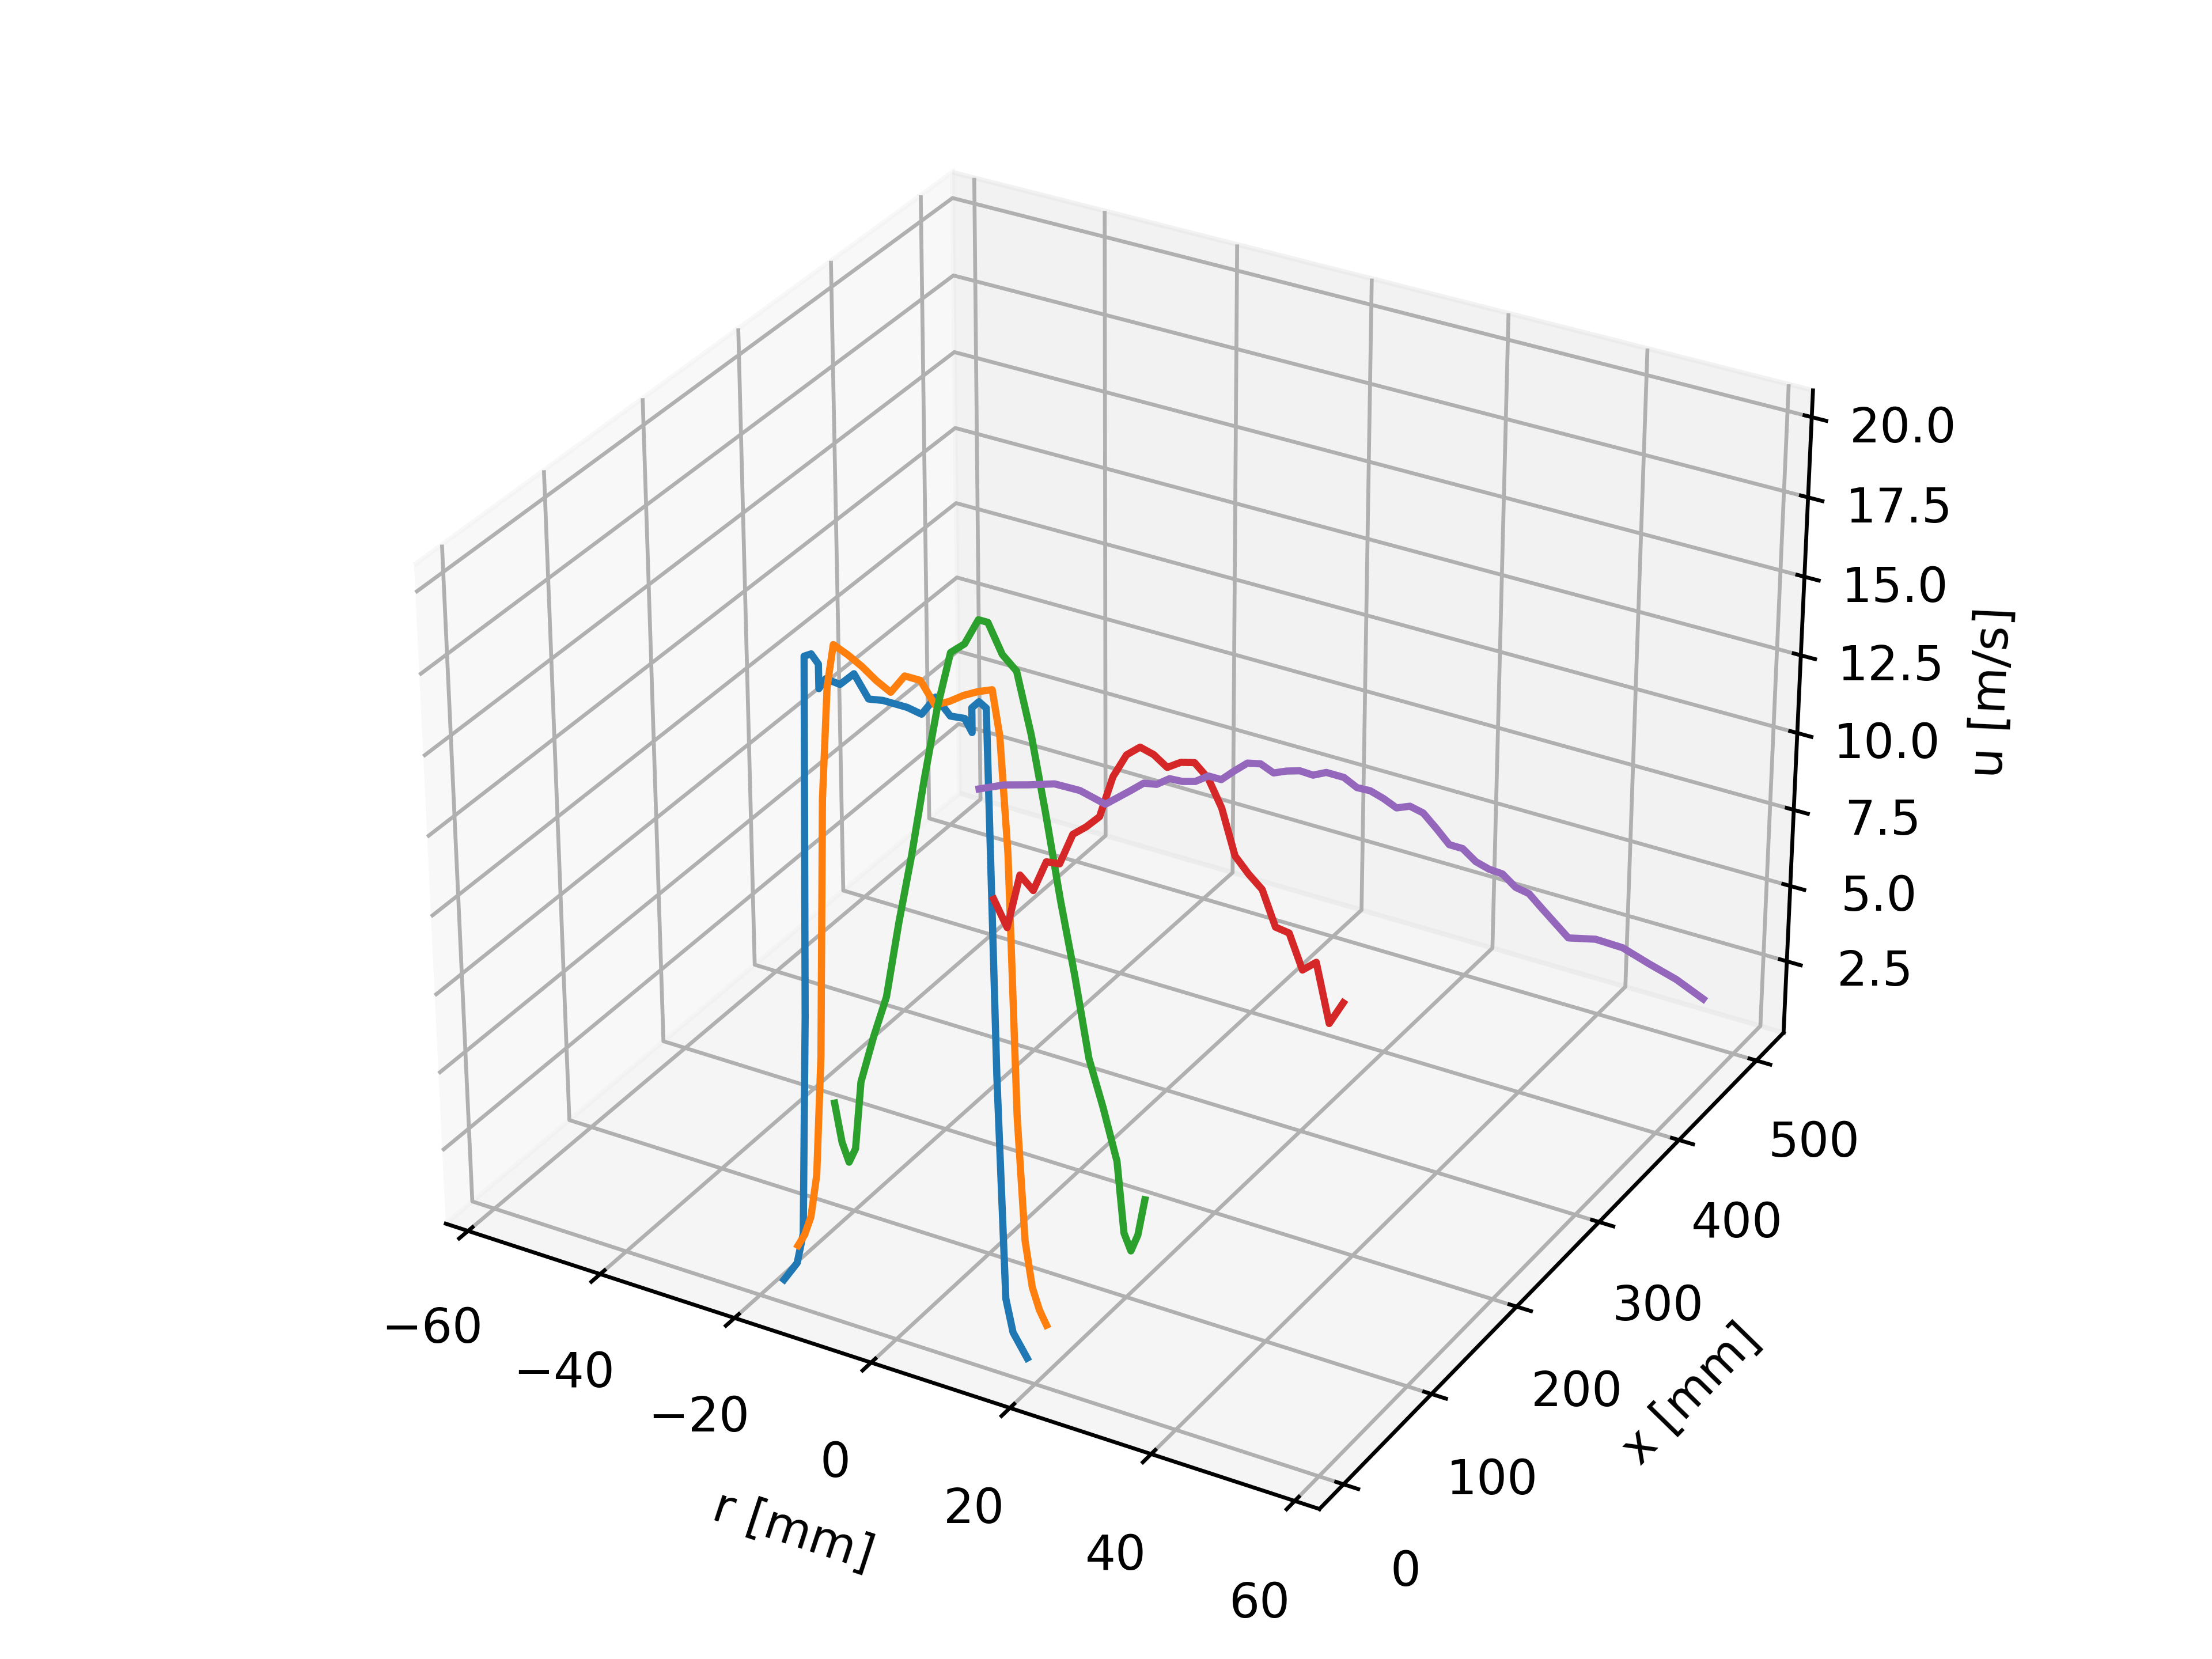
\includegraphics[width=.85\textwidth]{images/3/sq43d.png}
    \caption{Profili di velocità per la quarta squadra}
\end{figure}

\noindent Si evidenziano degli effetti spuri in prossimità dell'asse del getto, in particolar modo nel getto relativo alla quarta squadra. Questi possono essere dovuti a vari fattori, come ad esempio un non perfetto allineamento della slitta assiale con l'asse del getto. Tali effetti sono mitigati come indicato nel codice Python in appendice \ref{b3}.\\\\
Si nota come in prossimità dell'orifizio i profili di velocità presentano un tratto rettilineo. Tale caratteristica mette in mostra il cuore potenziale del getto, in cui la velocità è costante. Pertanto, si può ricavare la velocità iniziale del getto:
\begin{equation*}
    U_0 = U(r=0, x=0)
\end{equation*}
Utilizzando tale velocità si calcola il numero di Reynolds per i quattro flussi in esame:
\begin{equation*}
    Re = \frac{\rho U_0 D_j}{\mu}
\end{equation*}
Questi corrispondono a 15905, 26321, 42207 e 34102.\\\\
I profili di velocità che presentano una porzione del cuore potenziale del getto caratterizzano la mixing region del getto, mentre i profili successivi caratterizzano la zona di transizione e la zona self-similar.
\newpage
\noindent Si possono ora diagrammare i profili di velocità adimensionali, ad esempio normalizzando la velocità con la velocità iniziale del getto e la distanza radiale con il diametro del getto:
\begin{equation*}
    \frac U {U_0} = f\left(\frac r{D_j} \right)
\end{equation*}
\begin{figure}[H]
    \centering
    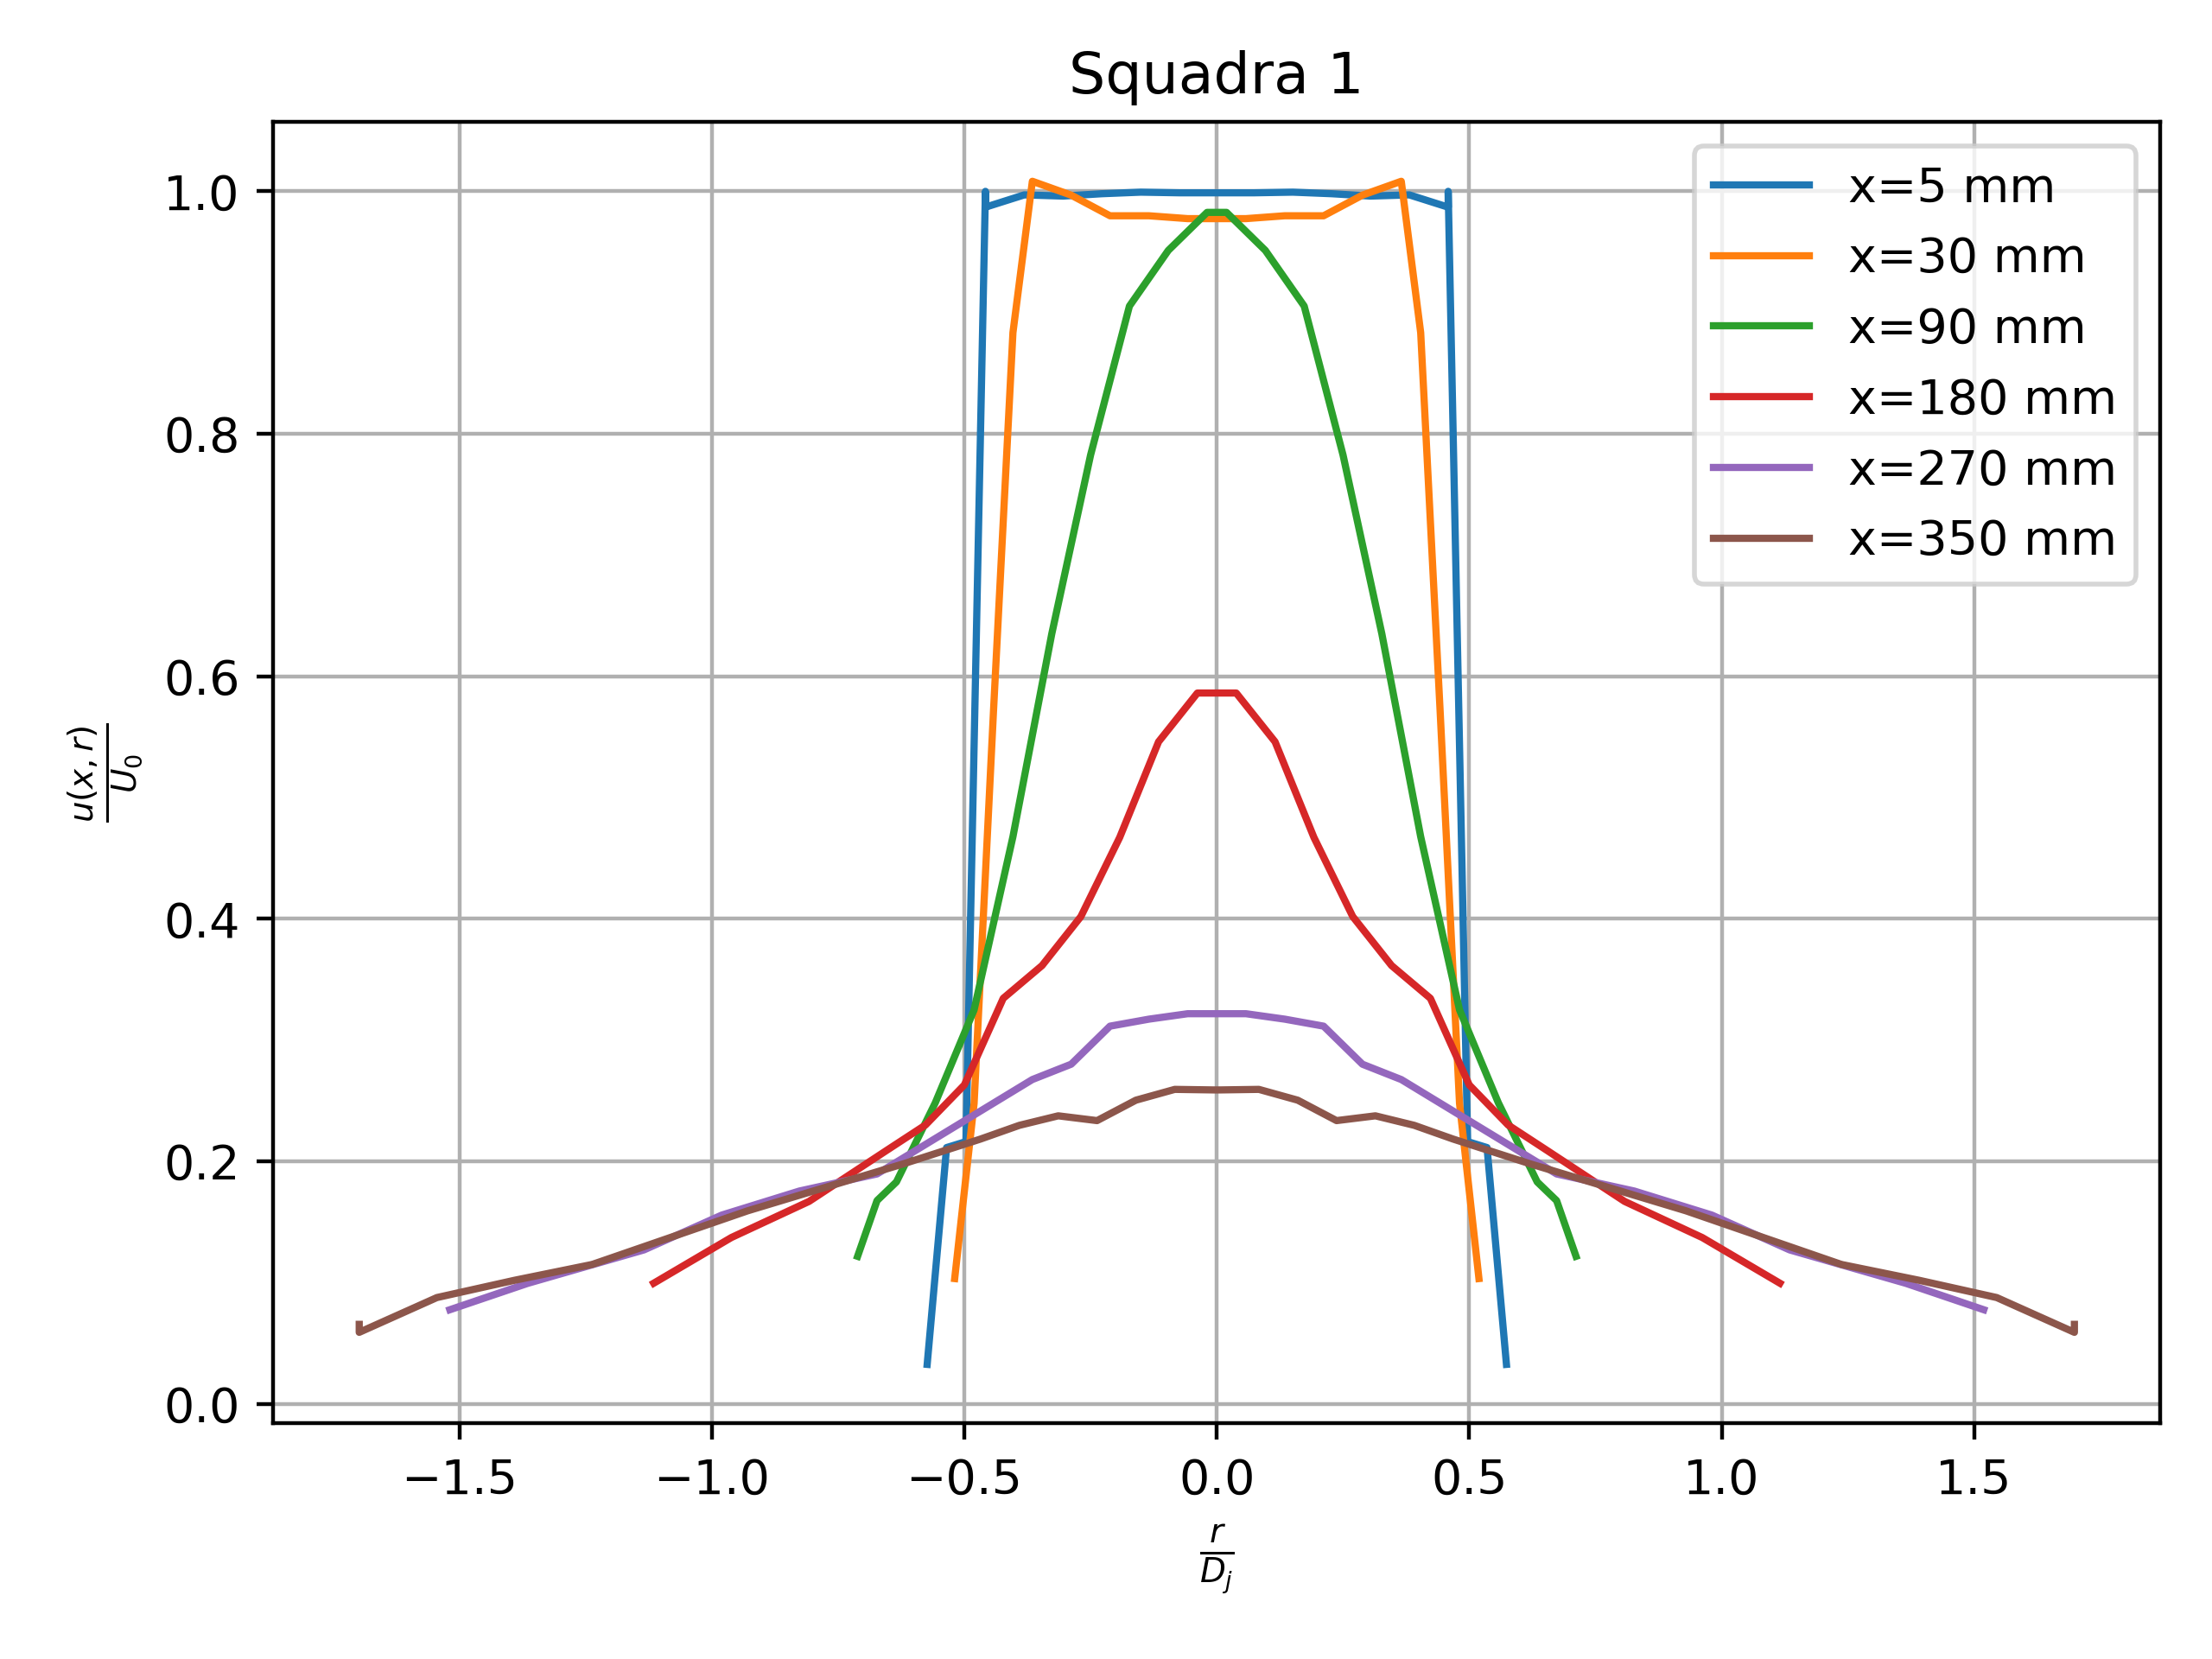
\includegraphics[width=.77\textwidth]{images/3/sq1u0.png}
    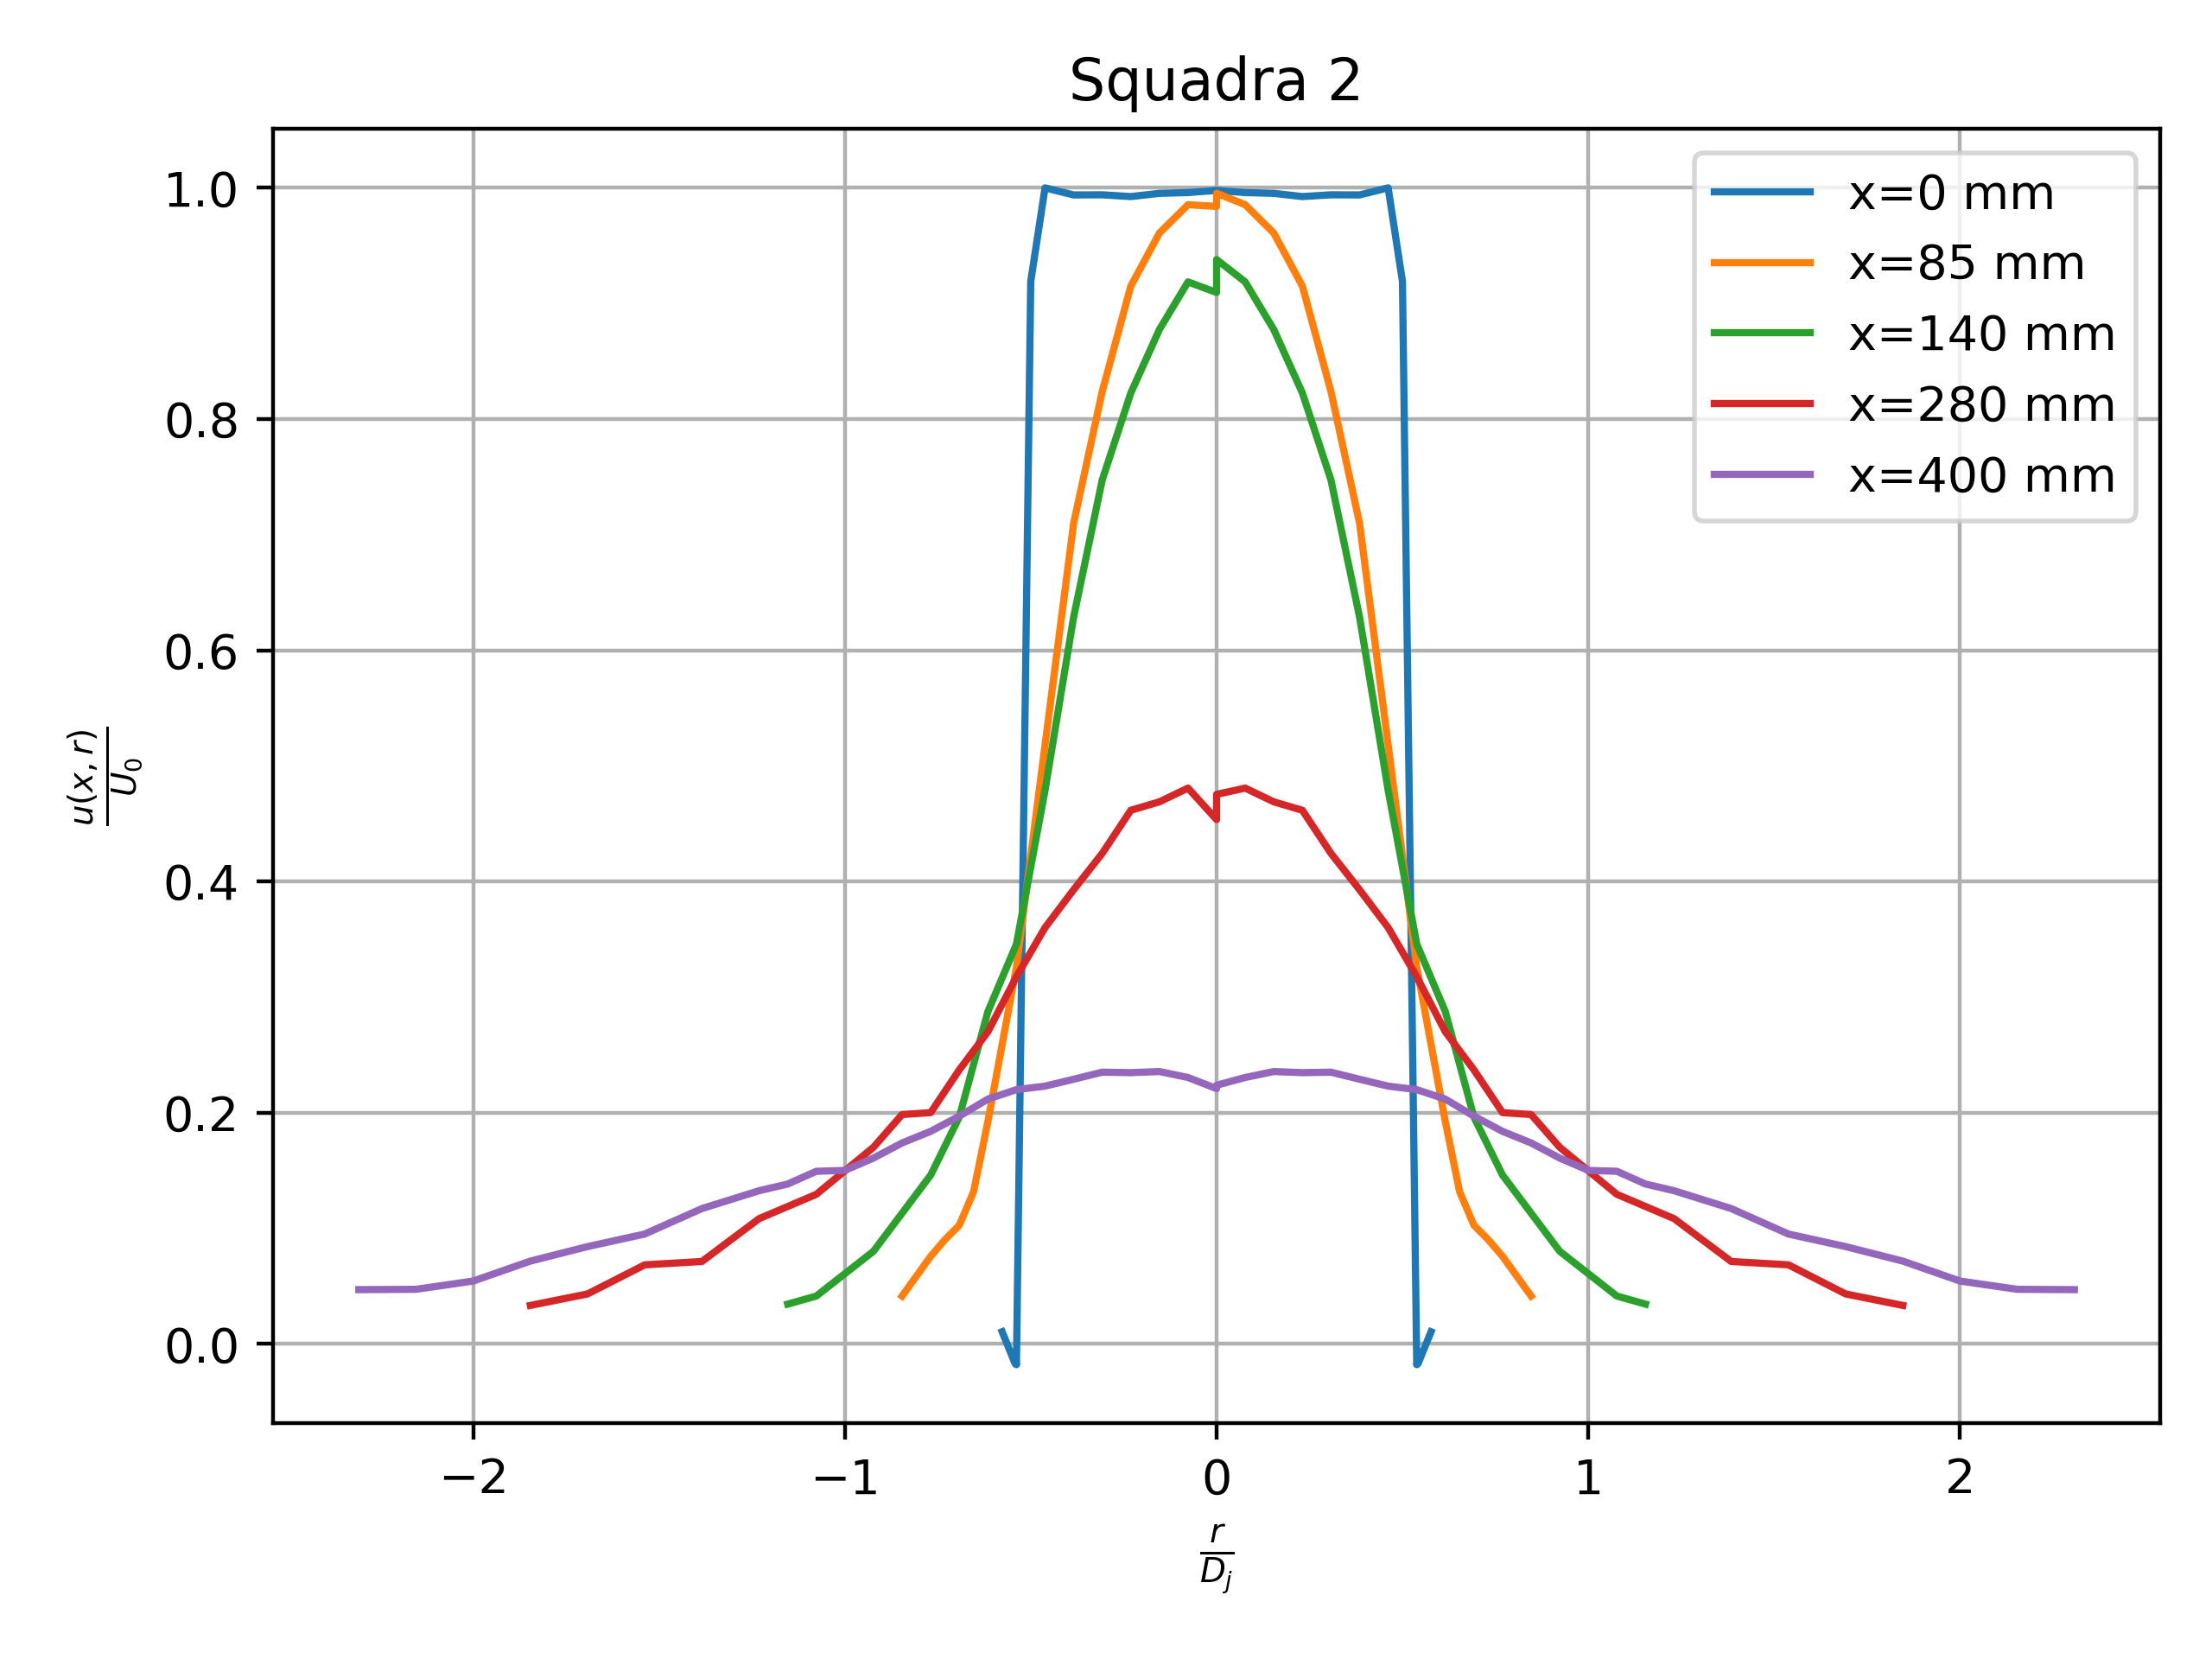
\includegraphics[width=.77\textwidth]{images/3/sq2u0.png}
    \caption{Profili di velocità adimensionali per la prima e per la seconda squadra}
\end{figure}
\begin{figure}[ht]
    \centering
    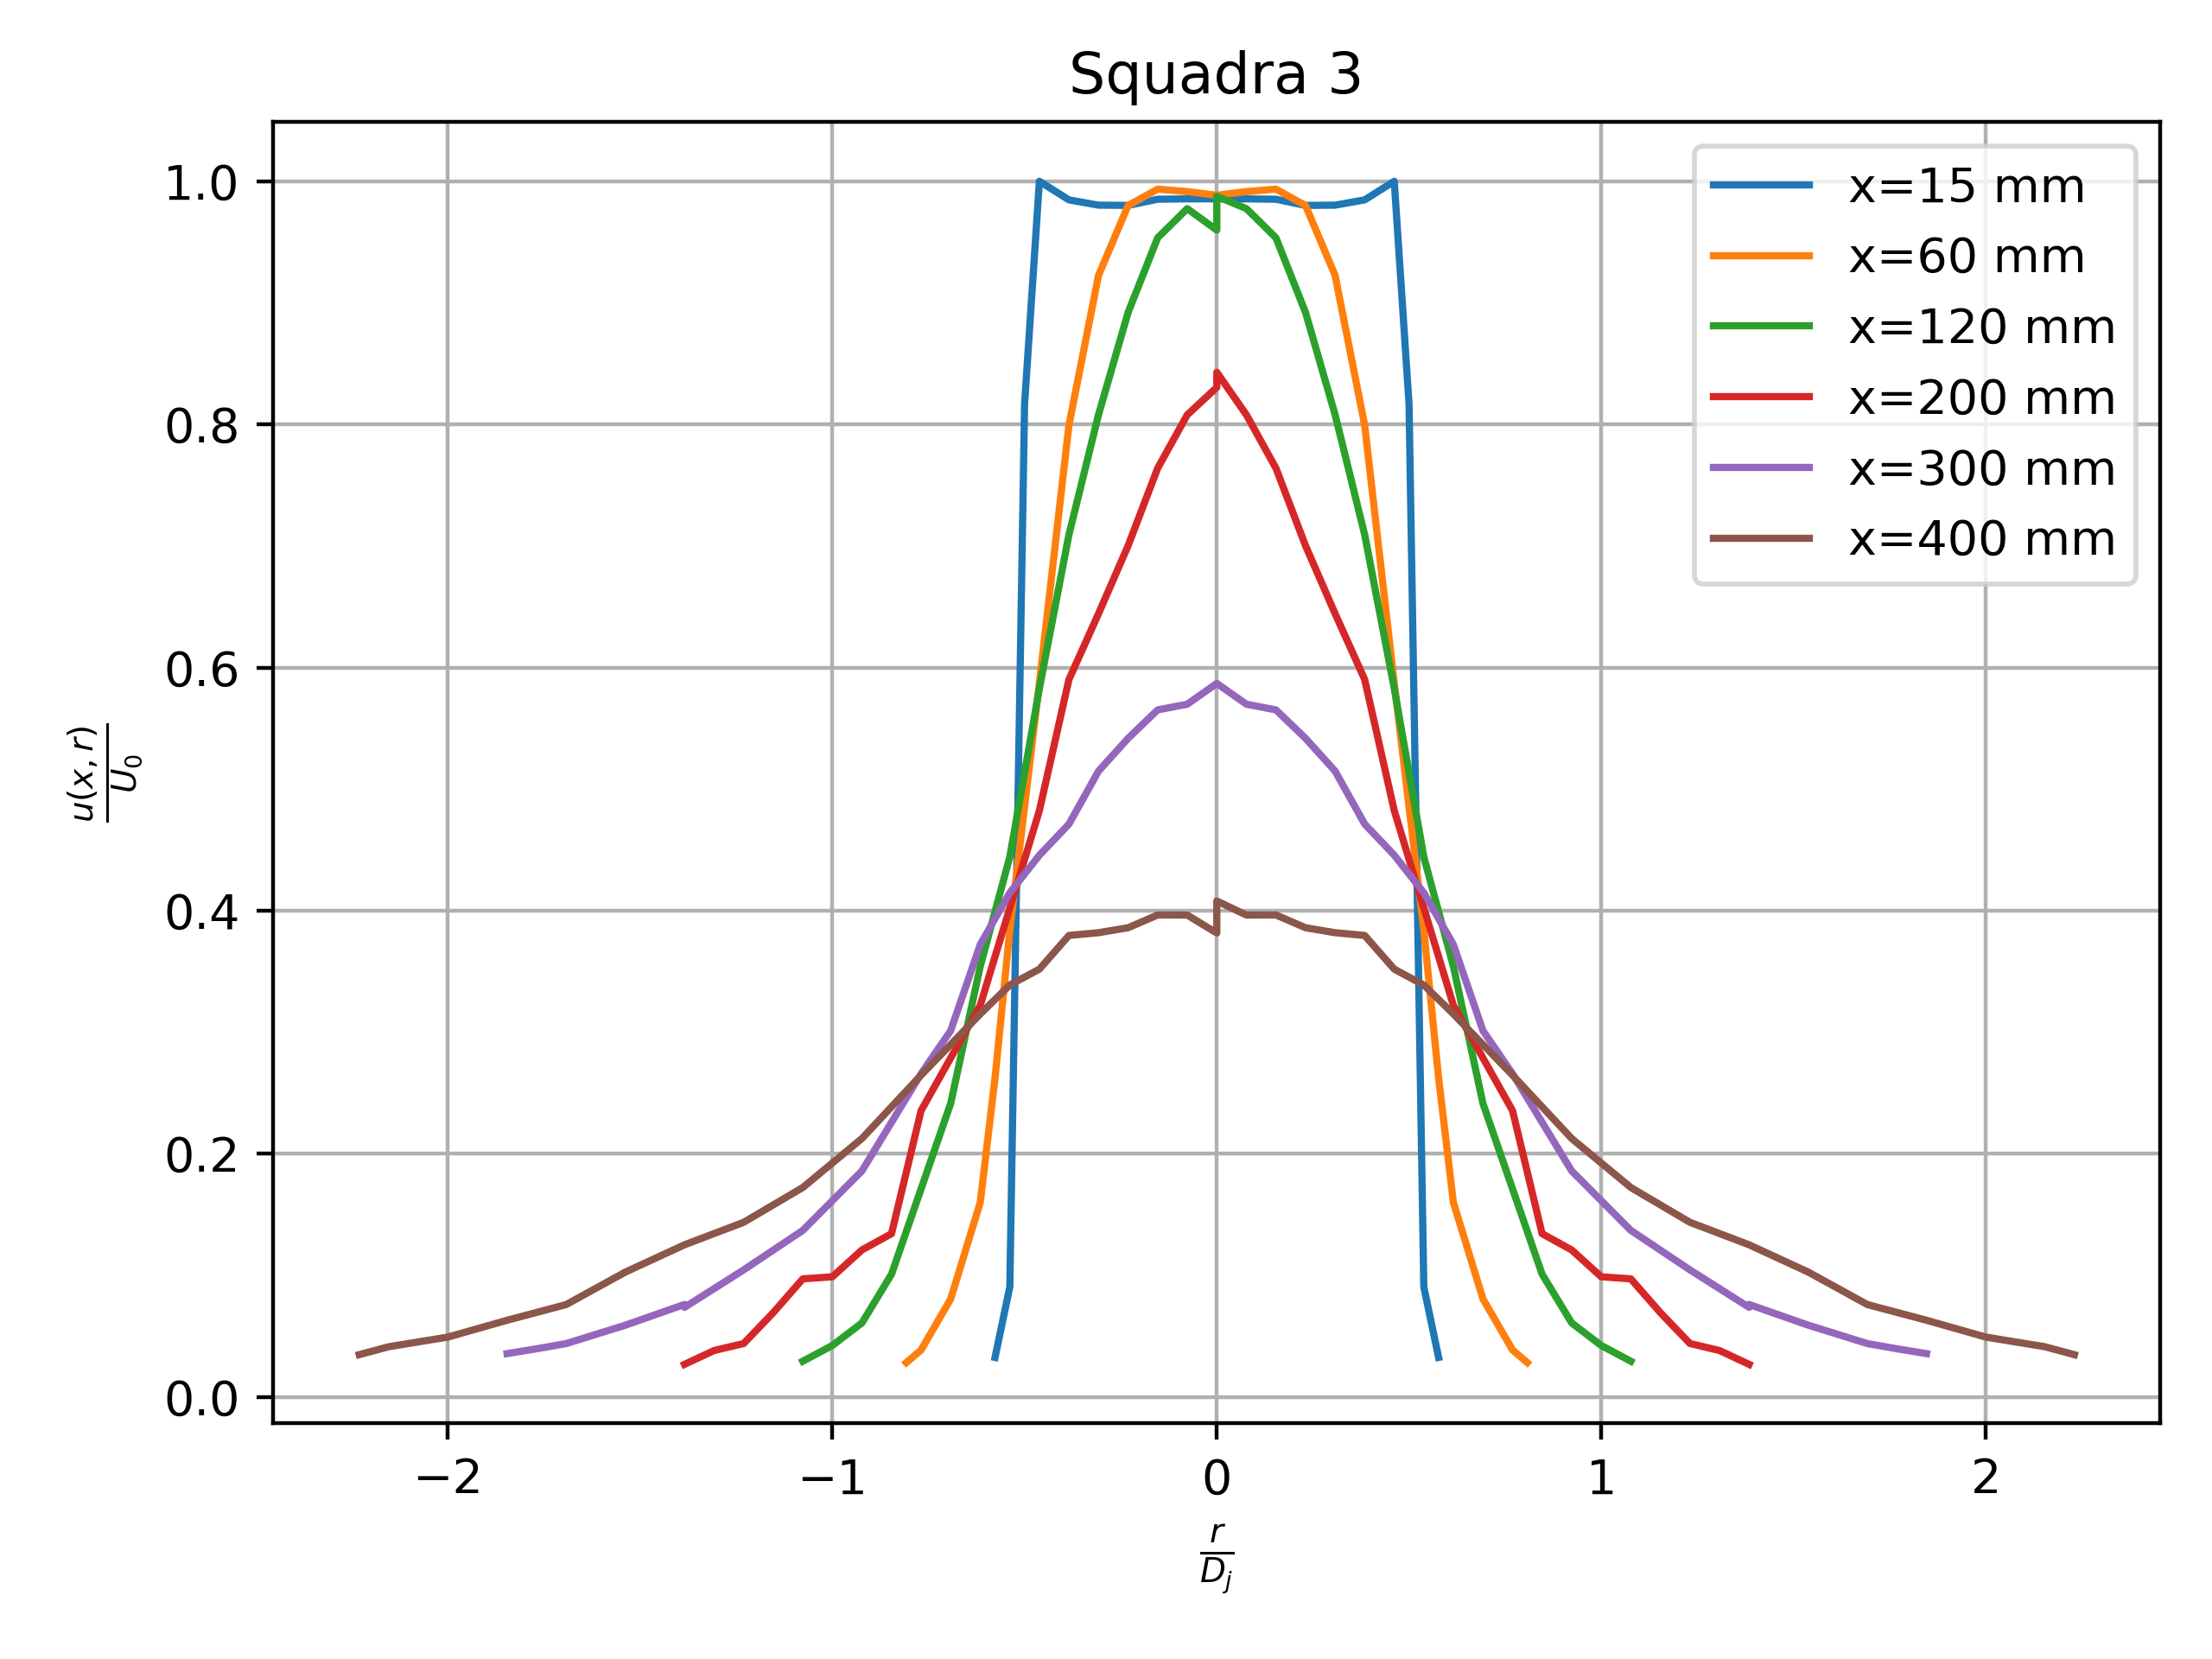
\includegraphics[width=.85\textwidth]{images/3/sq3u0.png}
    \caption{Profili di velocità adimensionali per la terza squadra}
\end{figure}
\begin{figure}[H]
    \centering
    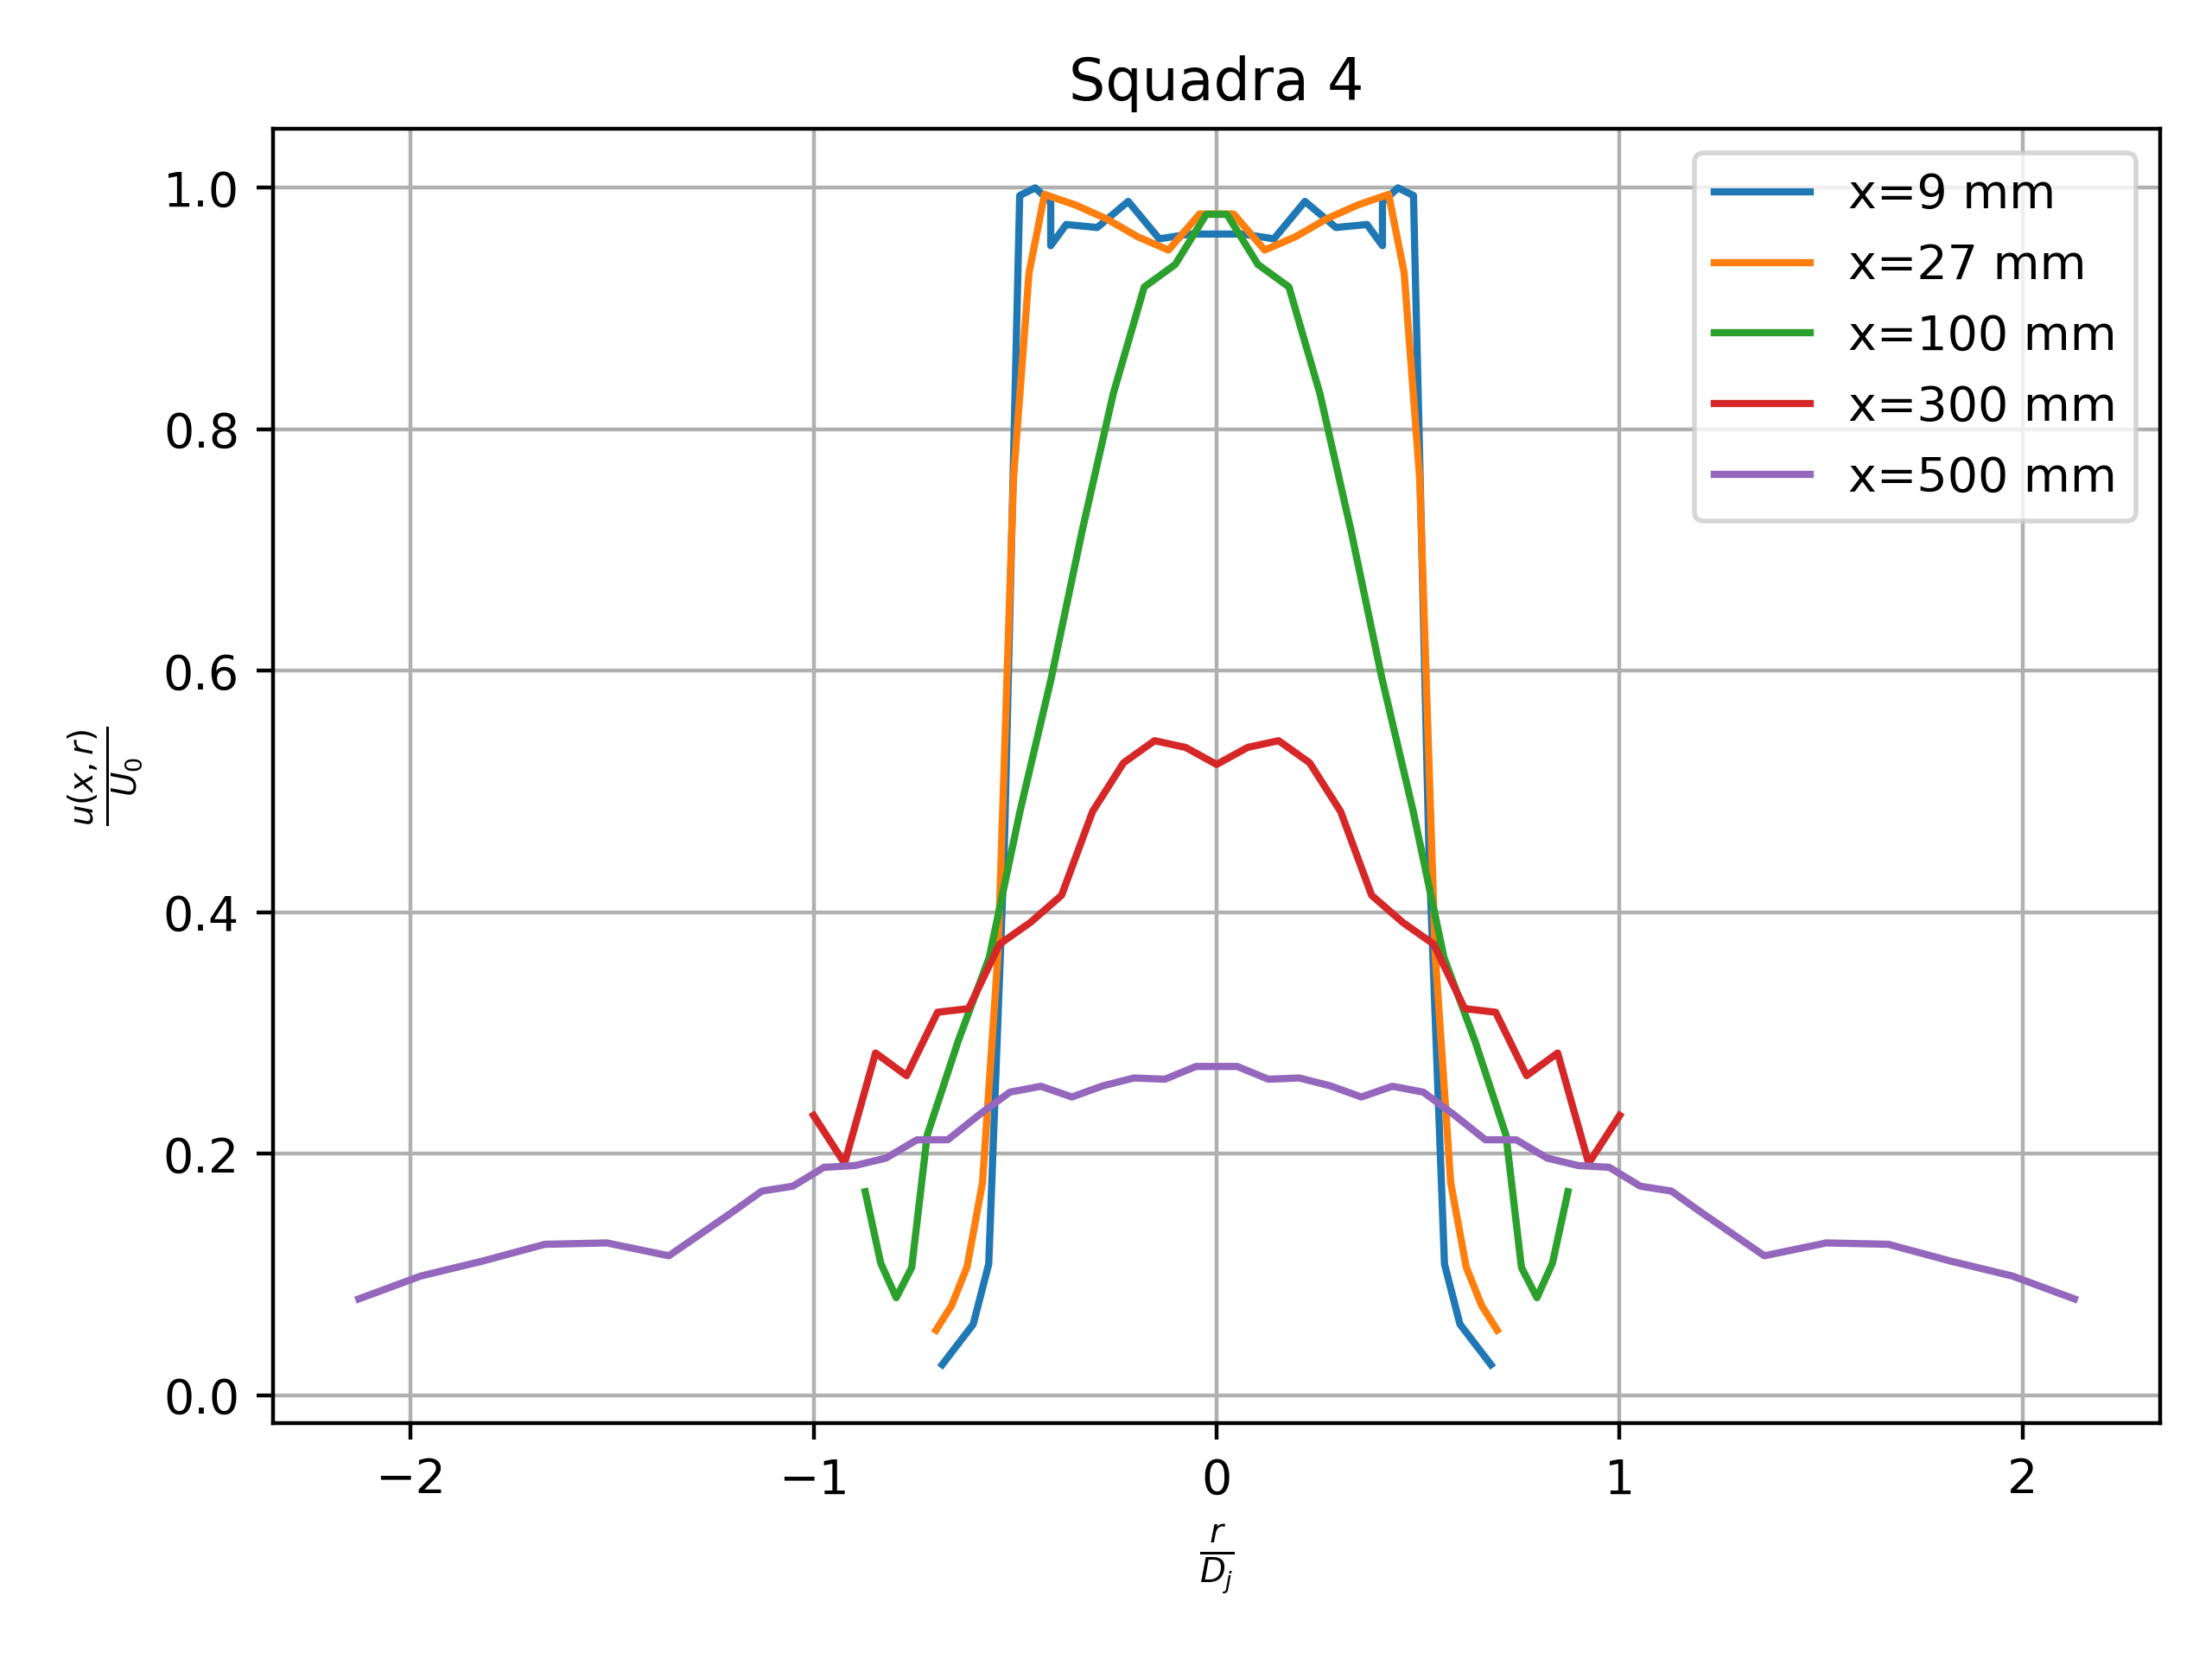
\includegraphics[width=.85\textwidth]{images/3/sq4u0.png}
    \caption{Profili di velocità adimensionali per la quarta squadra}
\end{figure}

\noindent Un ulteriore modo per diagrammare i profili di velocità adimensionali è quello di utilizzare la velocità massima locale e la dimensione trasversale del getto locale per normalizzare la velocità e la distanza radiale:
\begin{equation*}
    \frac{U(x,r)}{U_{max}(x)} = \frac{r}{r_{U=0.5U_{max}}(x)}
\end{equation*}
Il calcolo della velocità massima locale è immediato, per quanto riguarda invece la dimensione trasversale questa si calcola interpolando il valore di $r$ tale per cui la velocità è pari alla metà della velocità massima locale. Si ottengono quindi i seguenti diagrammi:
\begin{figure}[H]
    \centering
    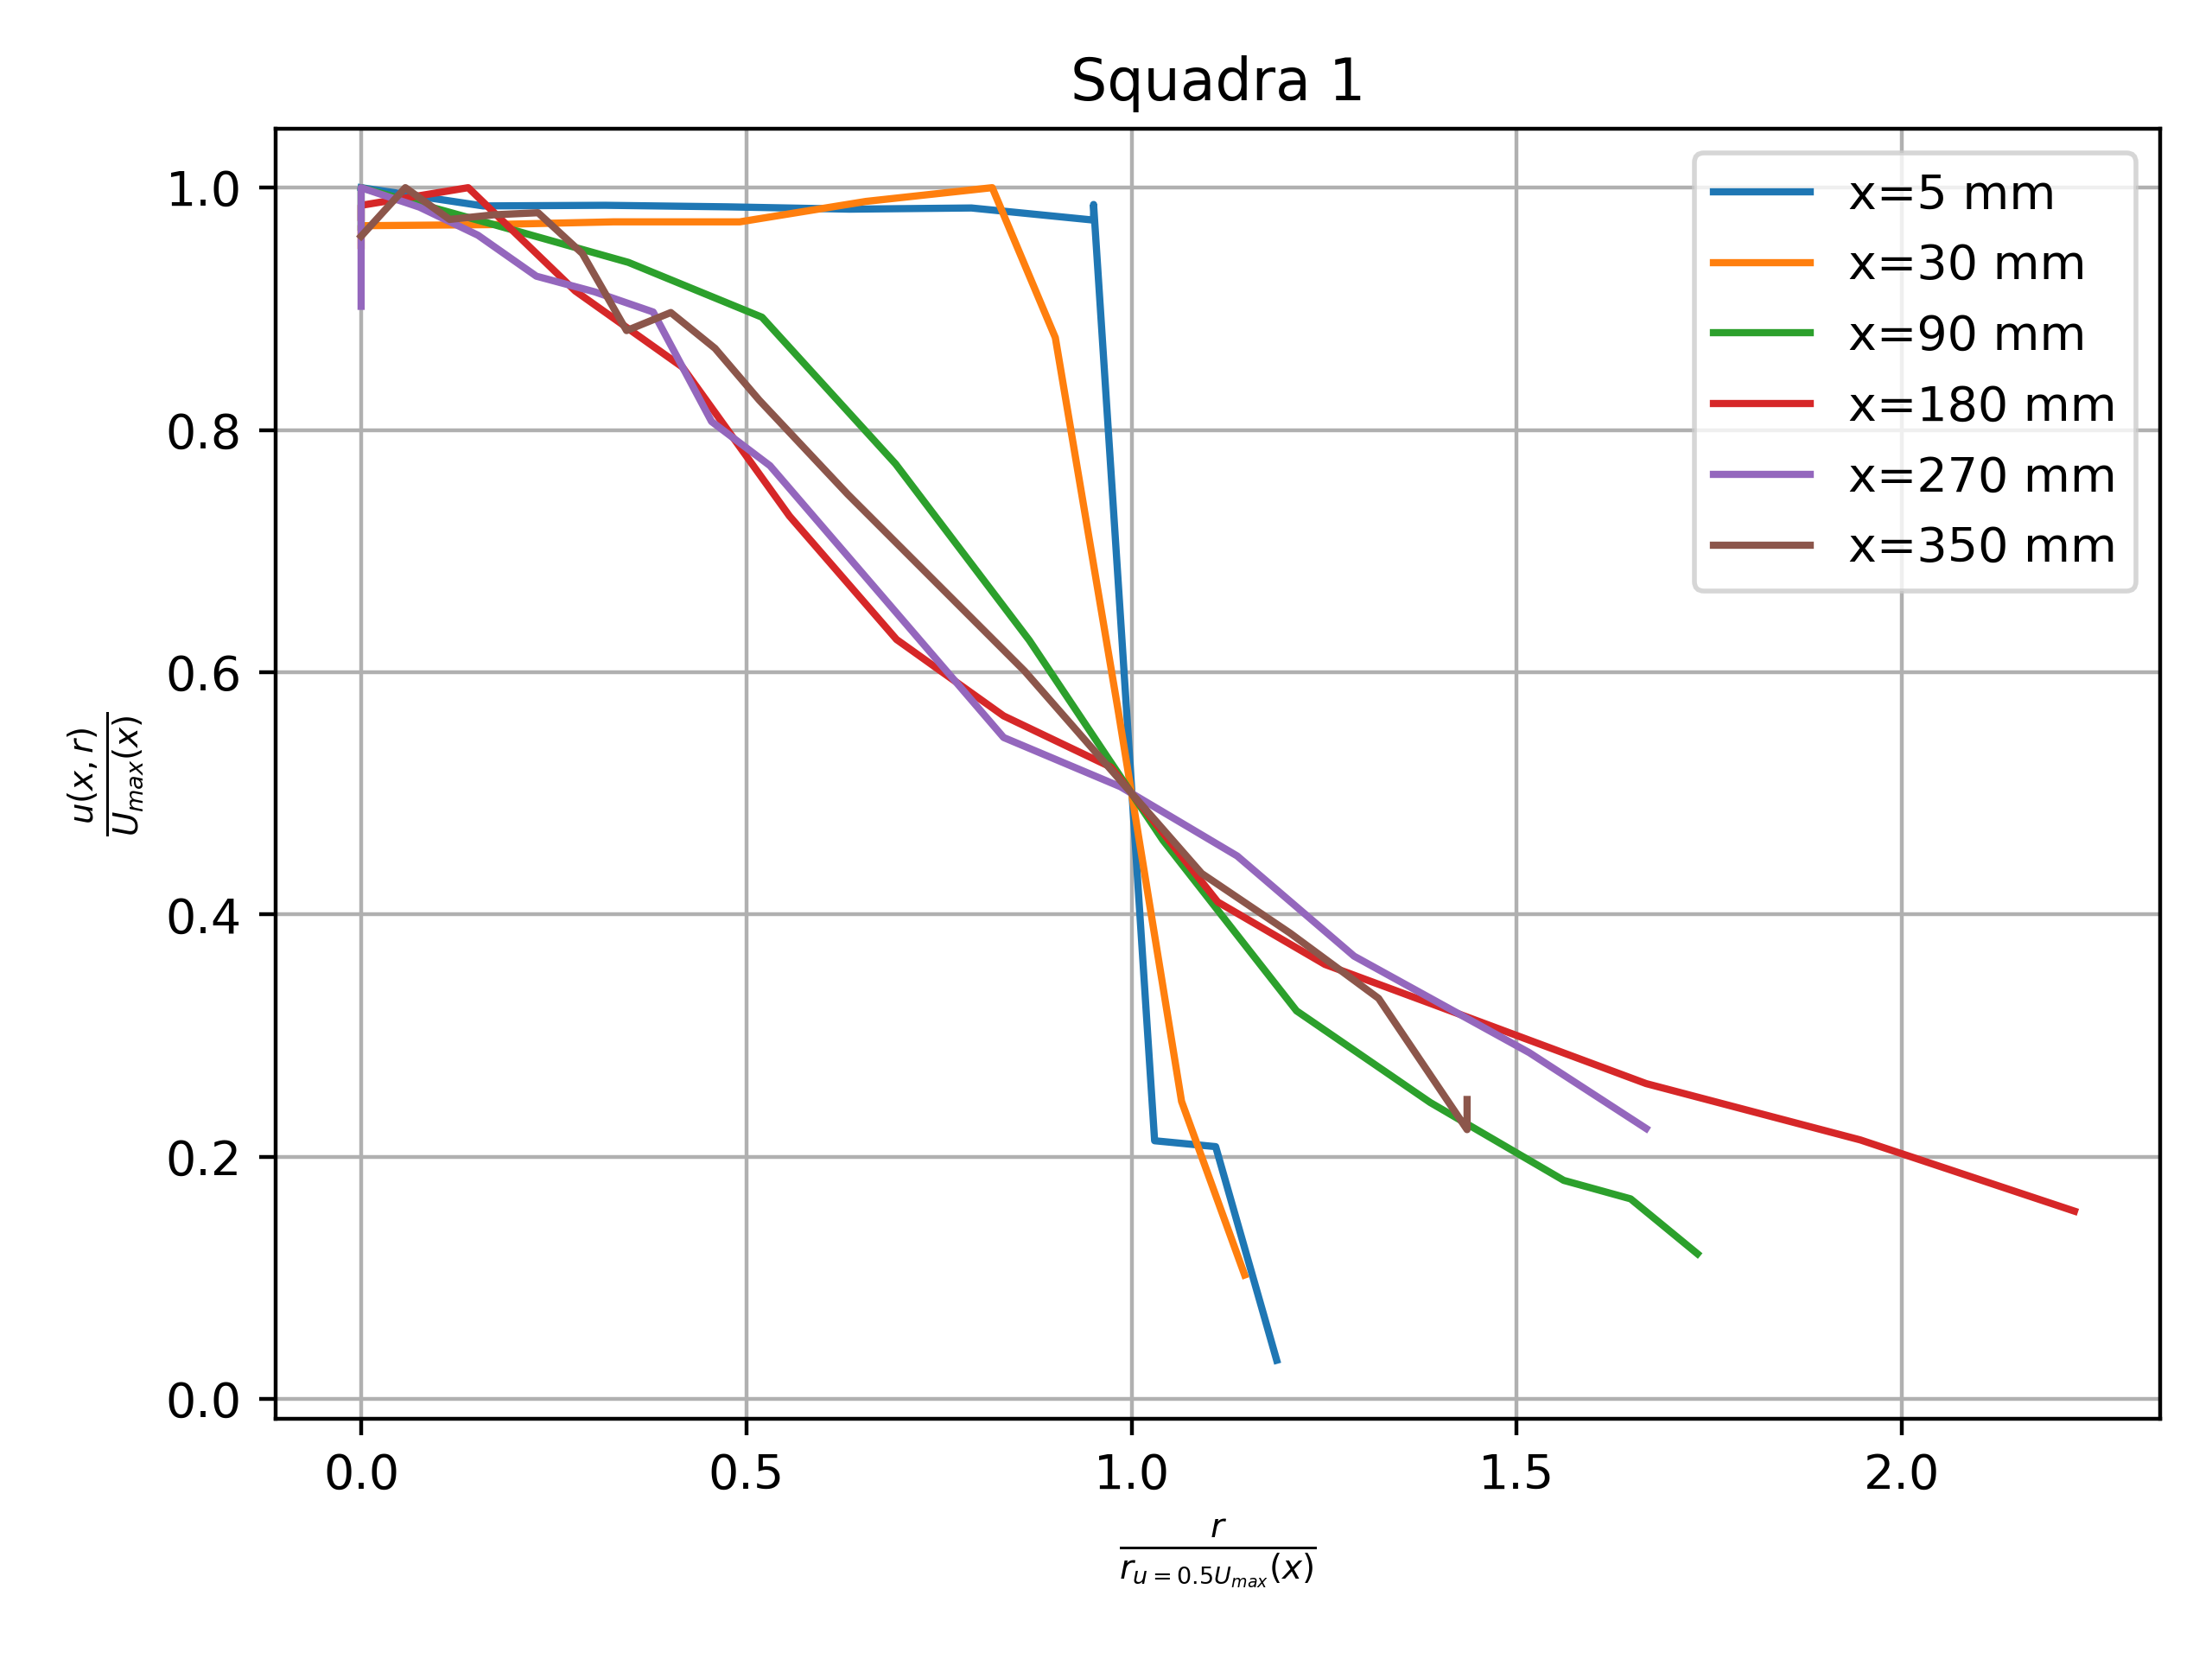
\includegraphics[width=.7\textwidth]{images/3/sq1umax.png}
    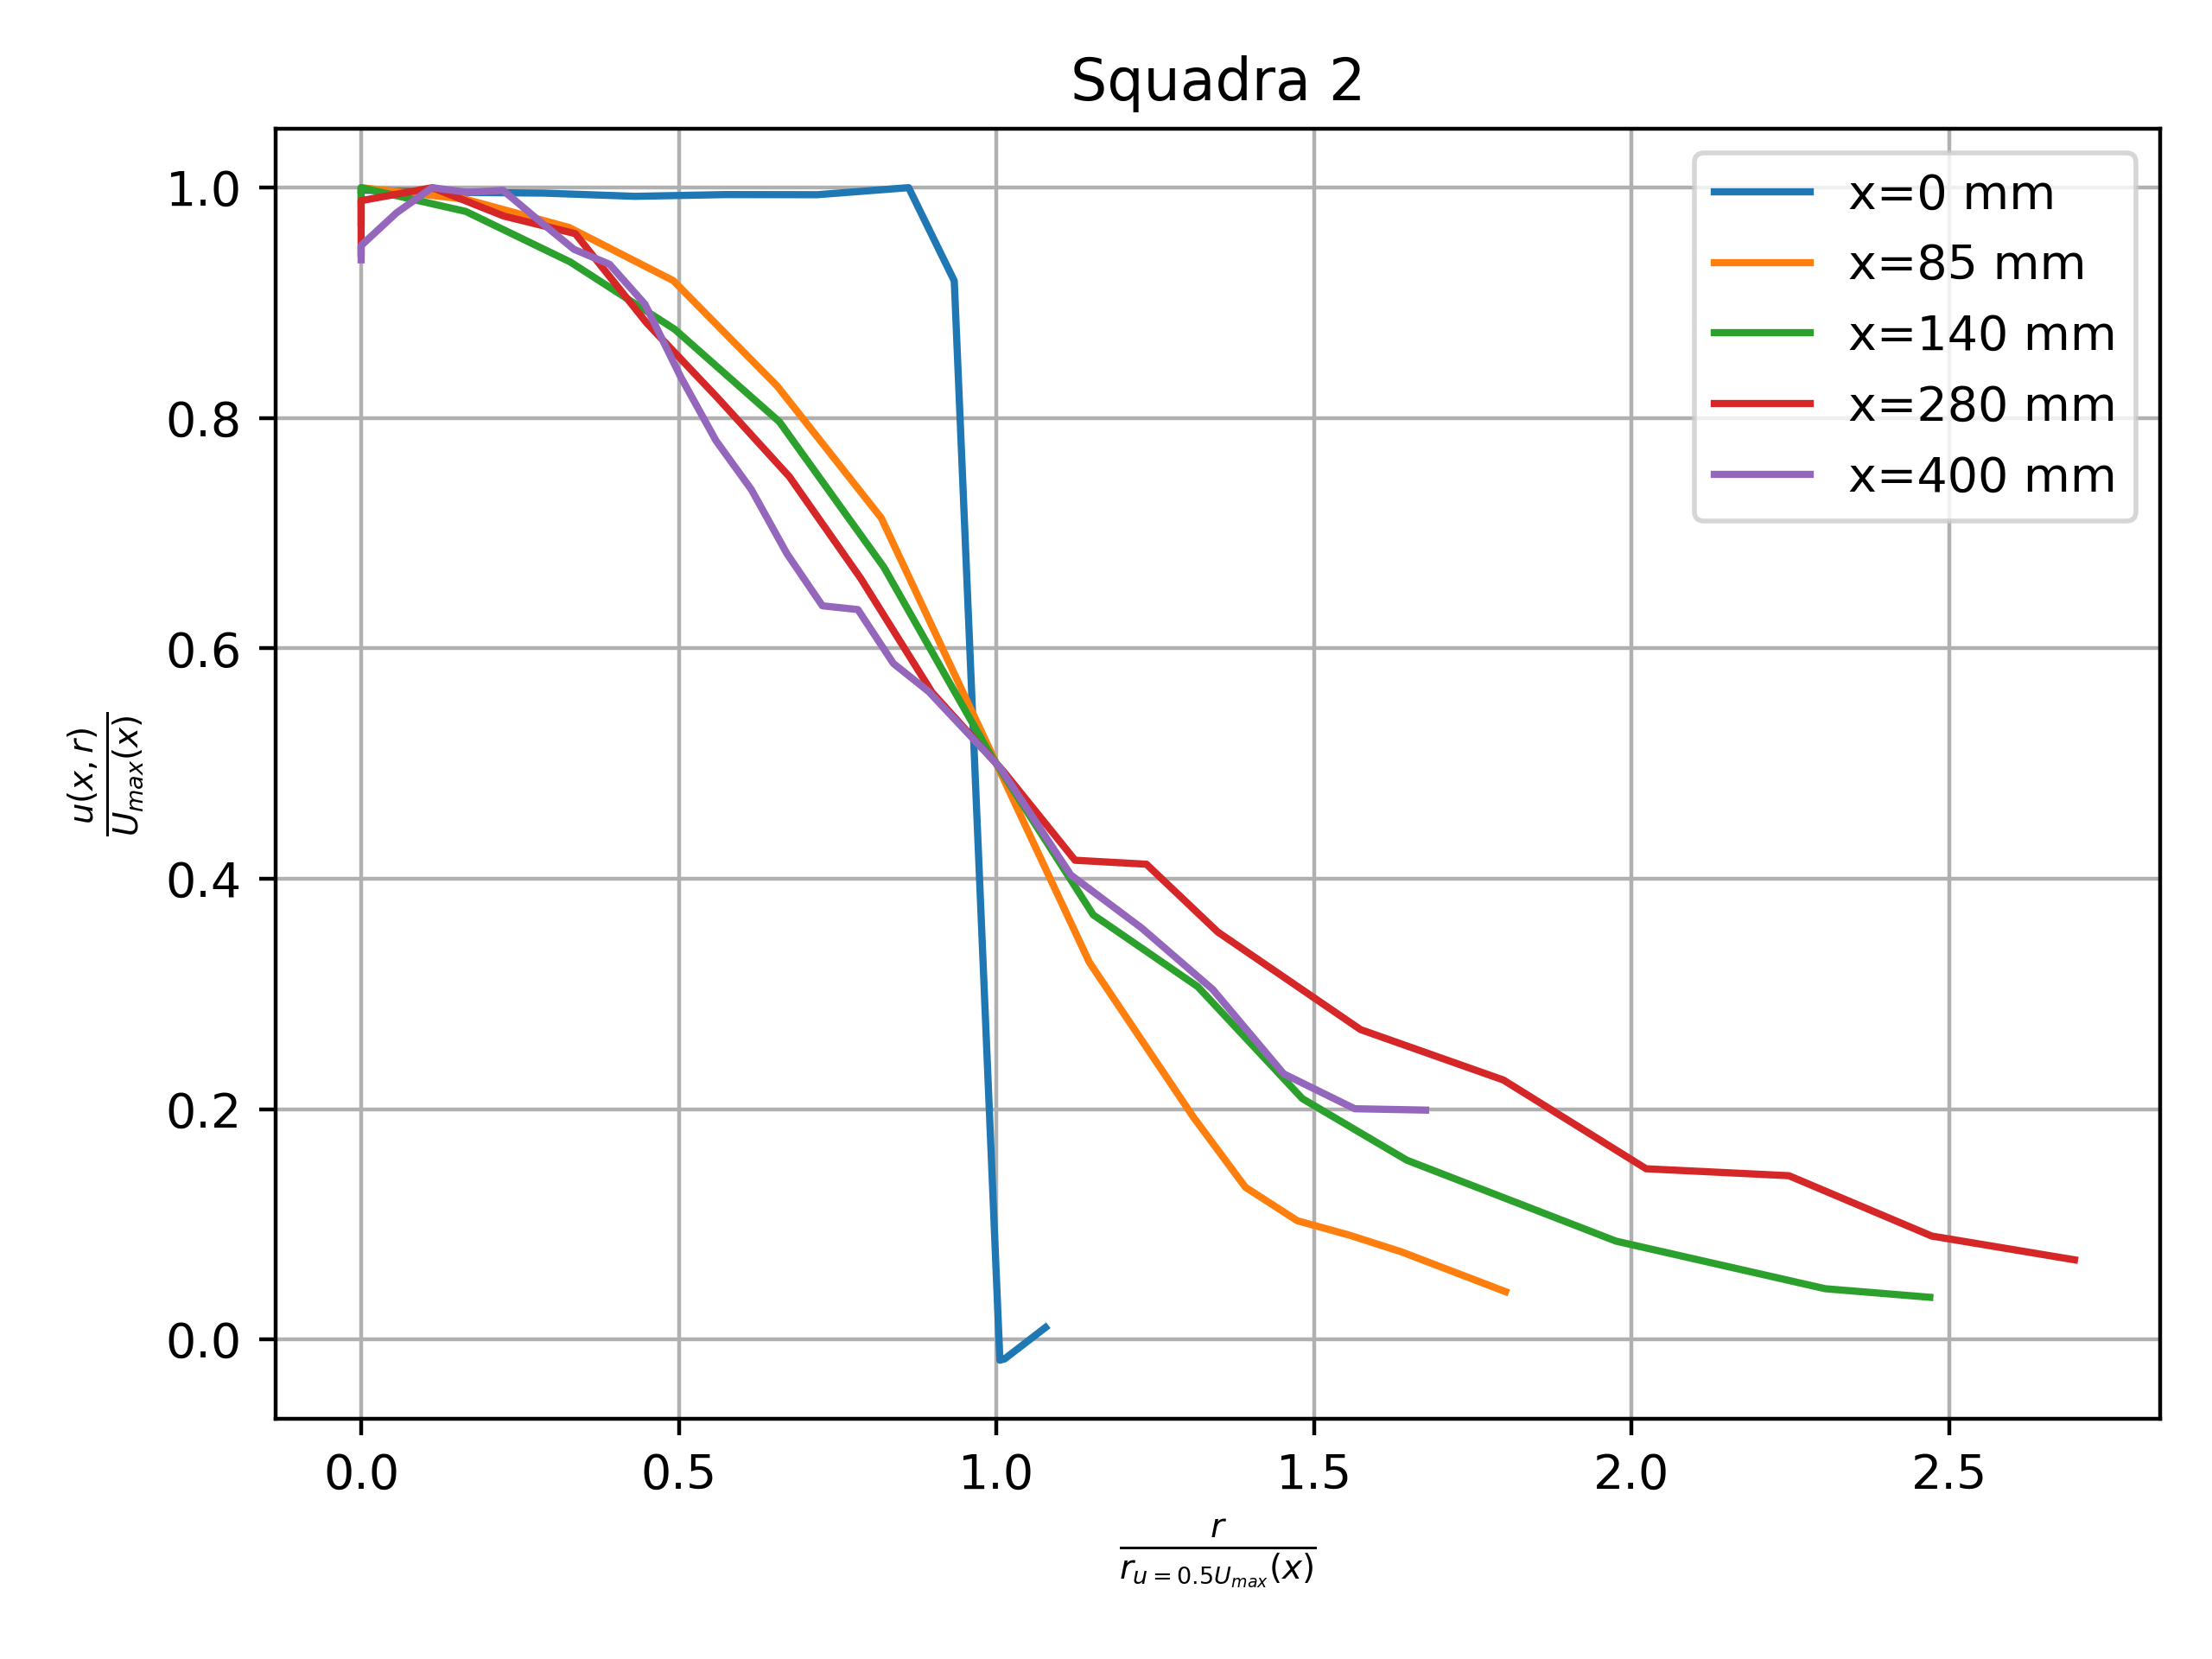
\includegraphics[width=.7\textwidth]{images/3/sq2umax.png}
    \caption{Profili di velocità adimensionali per la prima e per la seconda squadra}
\end{figure}
\begin{figure}[H]
    \centering
    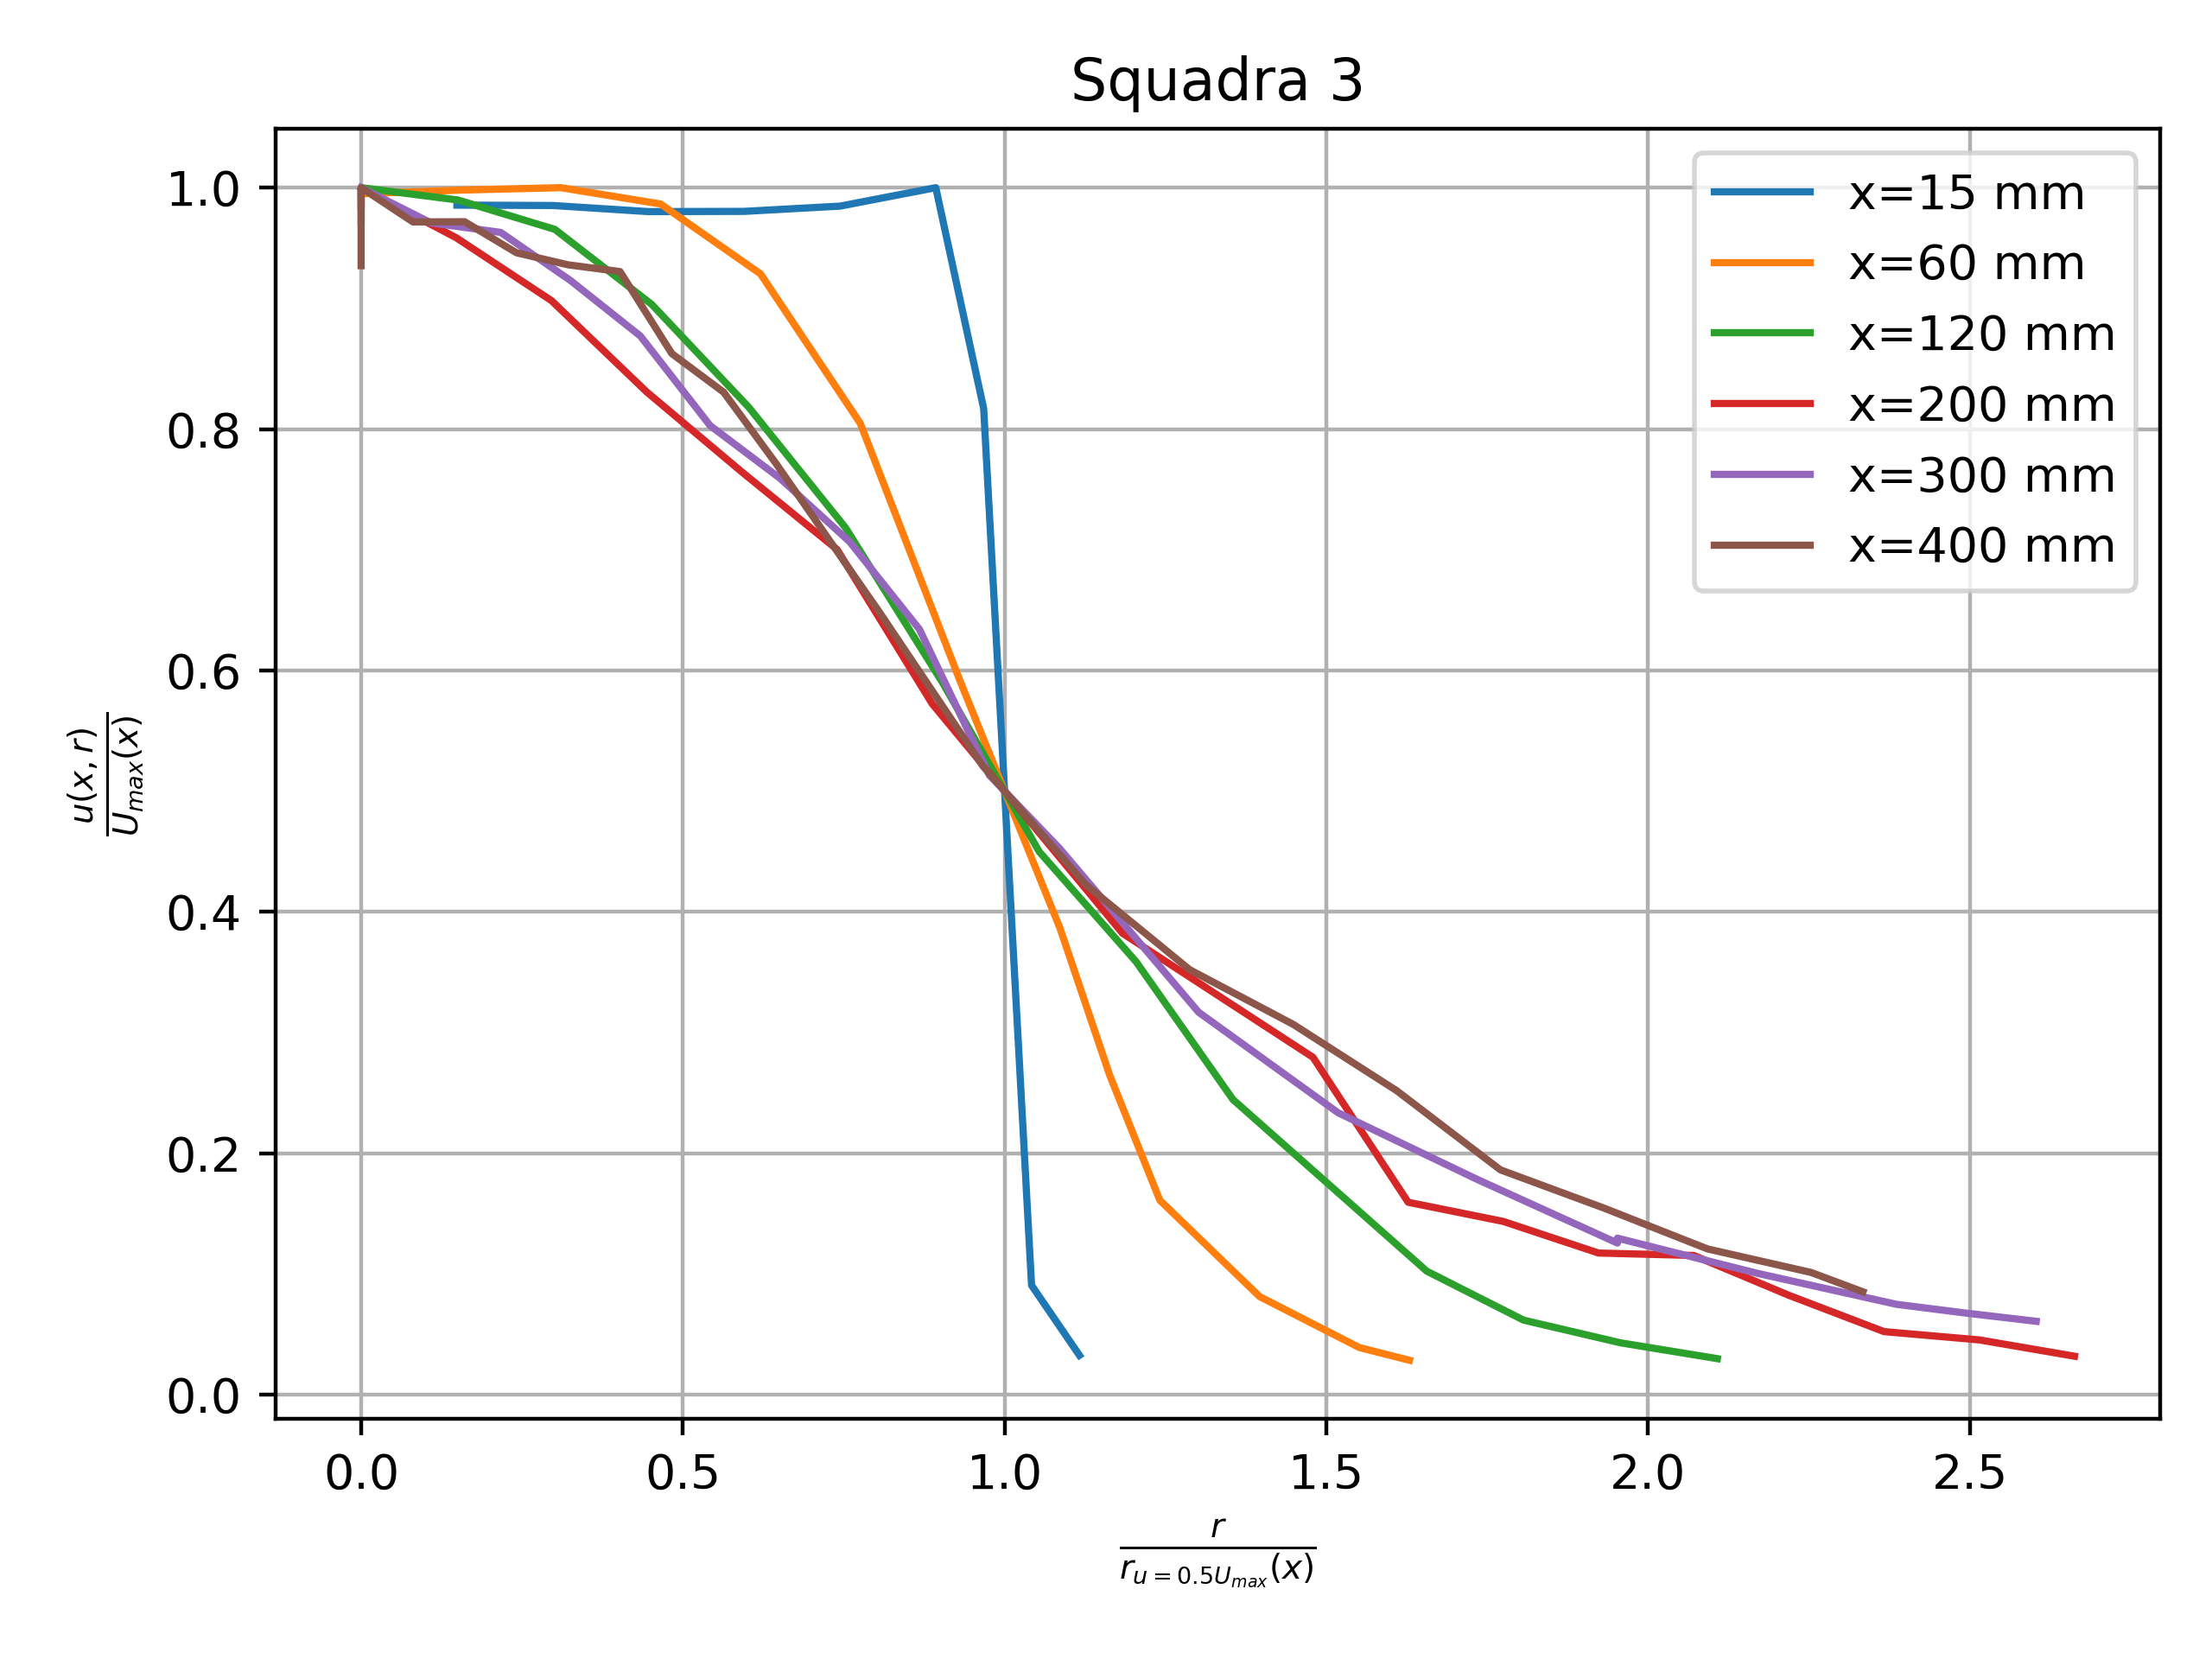
\includegraphics[width=.8\textwidth]{images/3/sq3umax.png}
    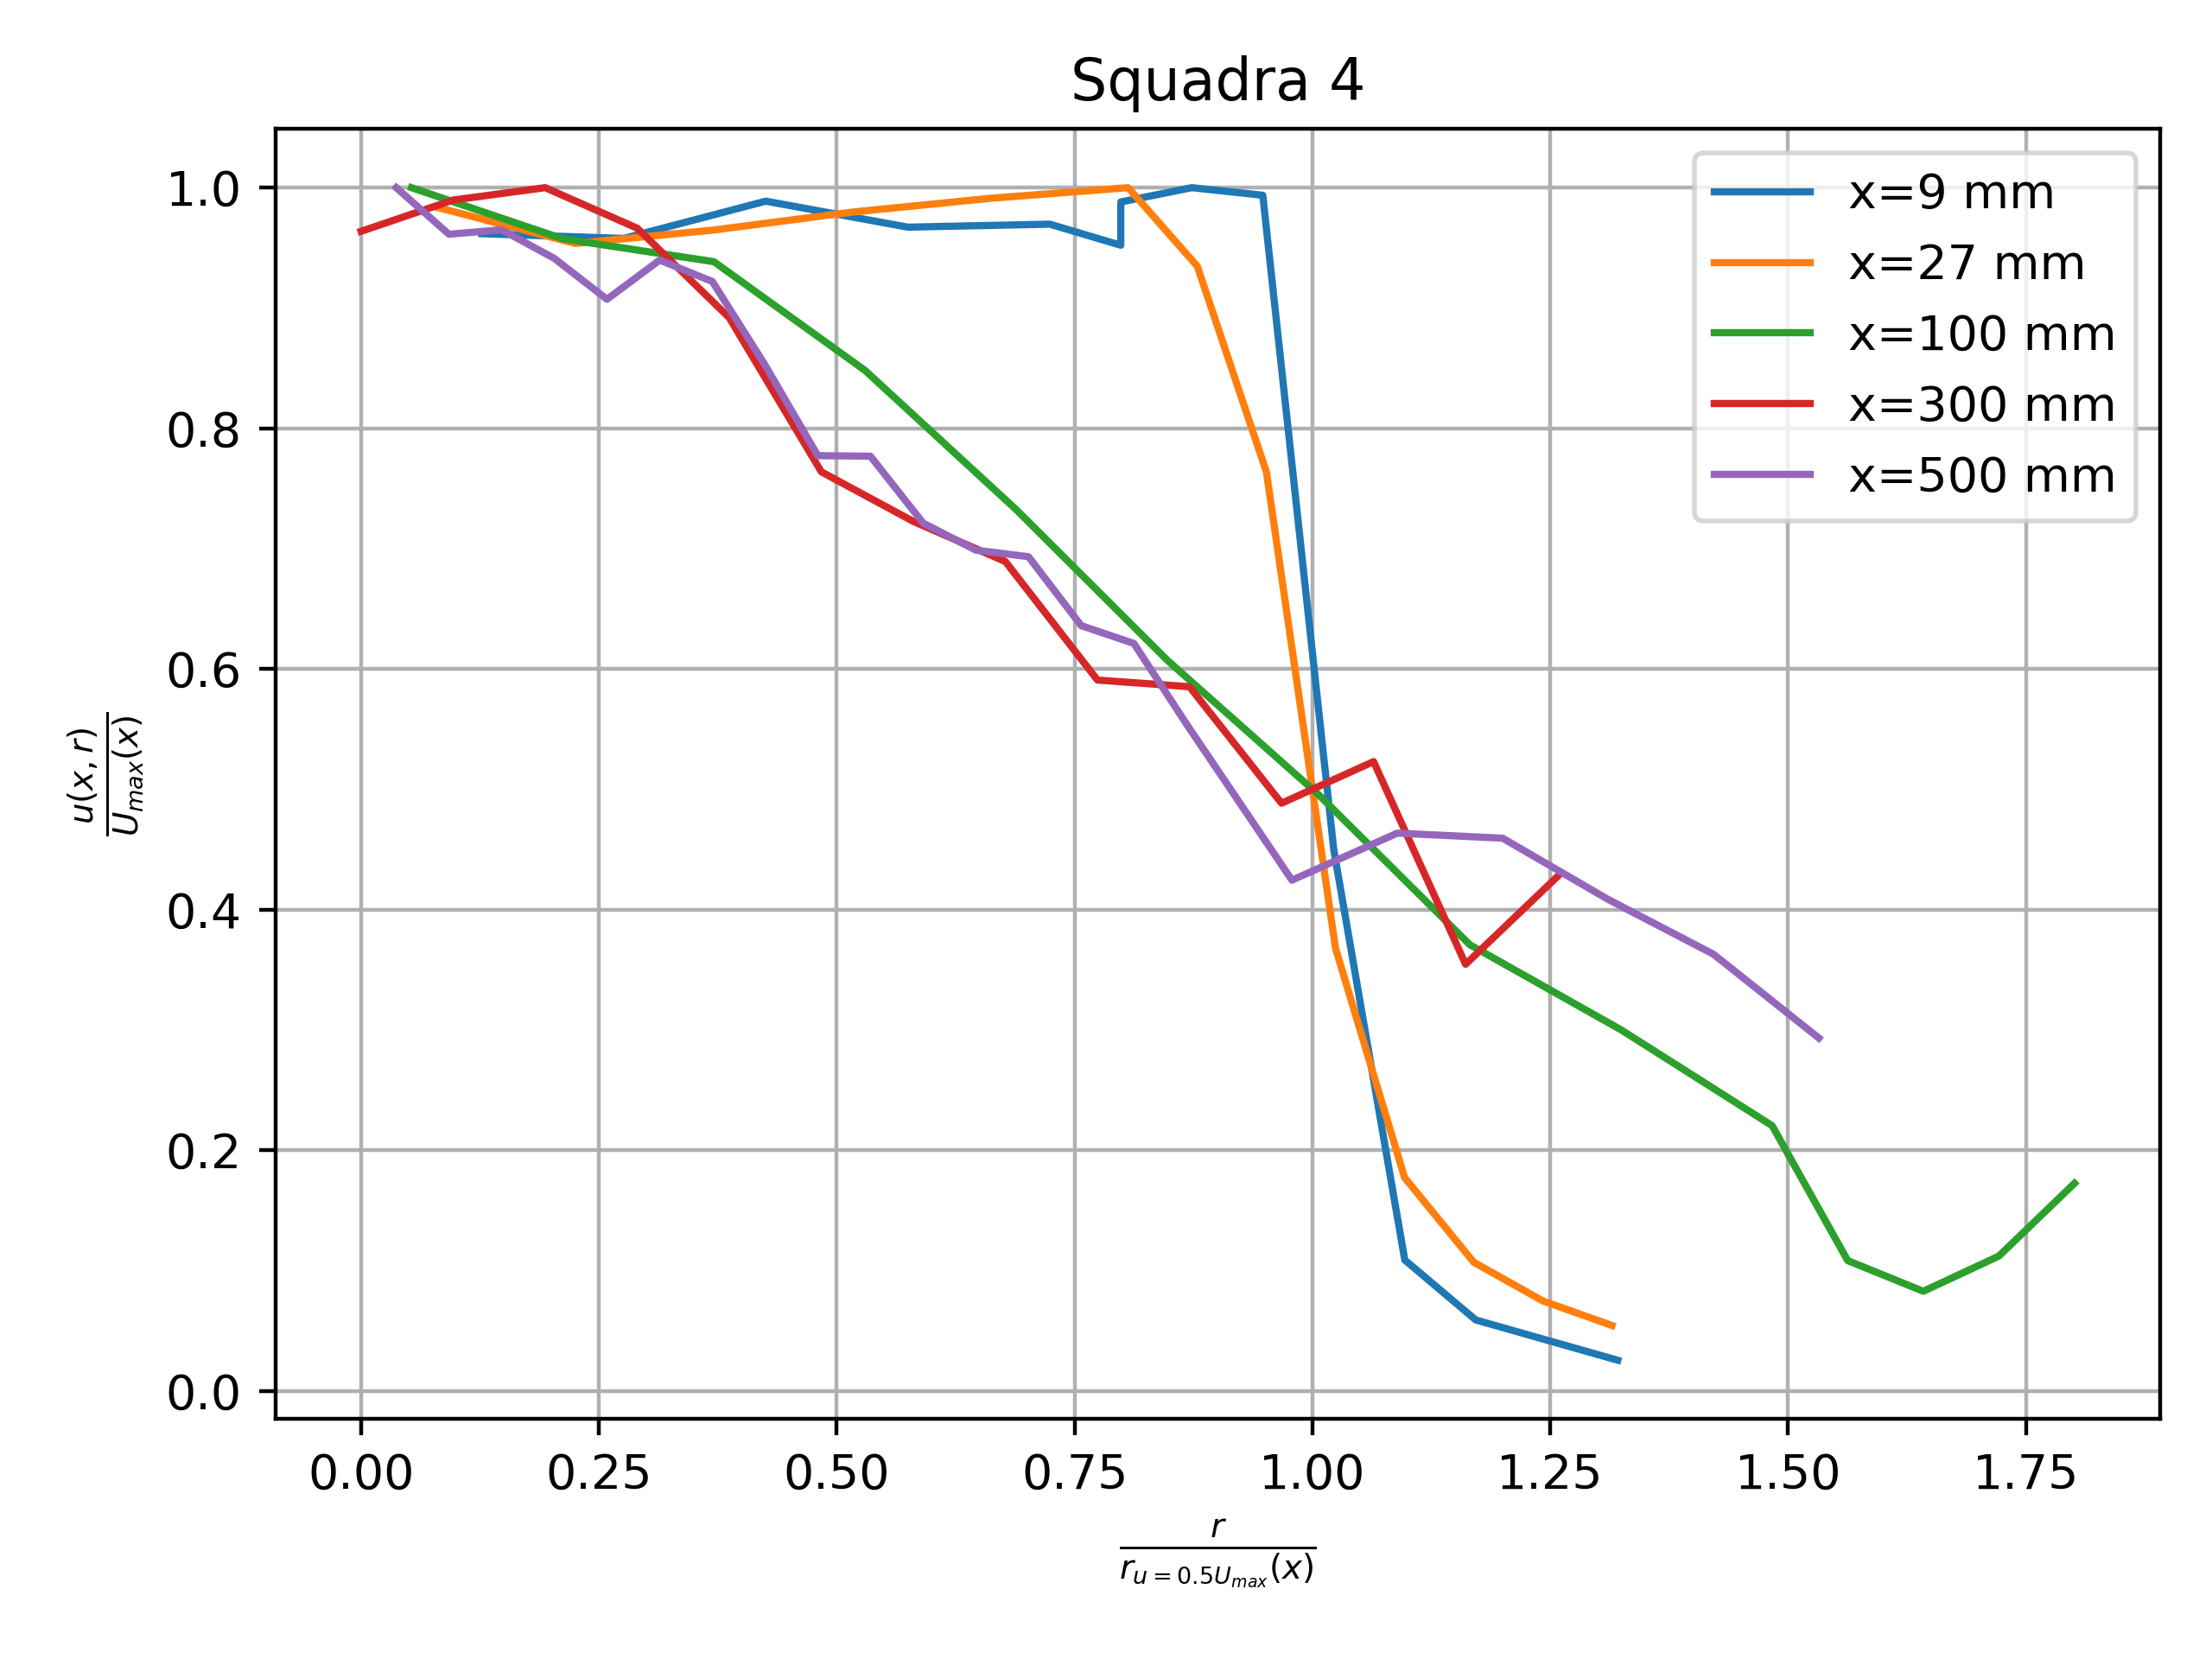
\includegraphics[width=.8\textwidth]{images/3/sq4umax.png}
    \caption{Profili di velocità adimensionali per la terza e per la quarta squadra}
\end{figure}

\noindent Così come accennato in precedenza, dai risultati ottenuti si osserva come nella regione autosimilare i profili di velocità adimensionali tendono a sovrapporsi.